\part{Managing Object Lifetime}

\chapter{Lifetime Requirements}
\index{Lifetime Requirements}

Your application needs some objects to live forever and it needs the rest to die
a timely death. Unfortunately, some of the important details governing memory
management are left in your hands. Java promised, with its automatic memory
management, that you could create objects without regard for the messy details of
storage allocation and reclamation. In Java, you needn't explicitly free objects,
which is at once the saviour from, and the source of, many problems with memory
consumption. Unless you are careful, your program will suffer from bugs such as
memory leaks\index{Memory Leaks} or excessive peak footprint. Furthermore, if
your objects don't easily fit into the limits of a single Java process, you will
need to manage, explicitly, marshalling them in and out of the Java
heap.\index{Marshalling}

Very often, your application uses a data structure in a way that falls into one
of a handful of common \emph{lifetime patterns}\index{Lifetime Patterns}. The
nature of each pattern dictates how much help you will get from the Java runtime
in the desired preservation and reclamaion of objects, and where it leaves you to
your own devices. \emph{A necessary step in the design process of any large
application is understanding into which lifetime pattern each of your data models
fit}. The five common lifetime patterns are: objects needed only transiently,
objects needed for the duration of the run, objects whose lifetime ends along
with a method invocation, objects whose lifetime is tied to some other object,
and, most difficult of all, objects that live or die based on need.
\autoref{tab:five-lifetimes} summarizes these five important patterns. We step
you through each of the patterns, defining them and giving examples of how to
know when you have an instance of each. In the next chapter, we show how to
implement these patterns.

%The trickier aspects of memory management, summarized in
%\autoref{tab:tricky-memory-management}, are discussed in greater detail in
%later chapters.

\begin{table}
\centering
	\begin{tabular}{lp{0.30\textwidth}p{0.35\textwidth}}
	\toprule  & Lifetime Property & Example \\ \cmidrule(r){2-2} \cmidrule(l){3-3}
	\autoref{temporary-lifetime}  & {Temporary} & new
	parser for every date
	\\
	\autoref{forever-lifetime} & {Needed Forever} & product catalog
	\\
	\autoref{correlated-lifetime-1} & {Correlated with Object}
	& object annotations
	\\
	\autoref{correlated-lifetime-2} & {Correlated with Phase} &
	DOM used only for parsing
	\\
	\autoref{deferred-deletion} & {Correlated with Need} &
	pooled Strings \\
%period\\ scoped to a phase/request\\
%correlated with an object (annotations)\\
%correlated with need}\\ \hline
%reusable & maybe i'll need it later \\ \hline
	\bottomrule
	\end{tabular}
	\caption{Five important categories of object lifetime.}
	\label{tab:five-lifetimes}
\end{table}

\section{Examples from a Server Application}

Configuring memory settings is an iterative process. It usually involves a
fair amount of trial and error, as one tunes the various knobs to balance memory
consumption and application performance. These knobs affect things like the size of the Java
heap, how many entries a cache should hold, and the timeout value for these
caches. This is usually a process of black box tuning: twist a knob, and see
how overall performance changes. In addition to being hit
and miss, it is also quite prone to bugs. If you set the size of a cache too
high, you risk poor performance due to excessive garbage collection, and even
possibly process failures, due to running out of heap space.

Tuning memory consumption in long-running applications, such as servers or
integrated development environments, is a particularly thorny issue. Improperly
managing memory in a short-running application may not be the end of the world.
In an application that runs more or less forever, mistakes can pile up over time.
In addition, they synthesize information from a diverse array of sources, each
with its own performance trade-offs. As such, caching plays a large role in these
applications. Consider an example from a server aplication.

\begin{example}{Object Lifetimes in a Server Application}
A web application commerce server preloads catalog data into memory to allow for
quick access to this commonly used data. It also maintains data for users as they
interact with the system, browsing and buying products. Finally, it 
caches the response data that comes from a remote service provider that charges
per request. How does Java heap consumption vary over time? Which heap size
fluctuations indicate a problem, and which are expected behavior?
\end{example}

\begin{figure}
	\centering
	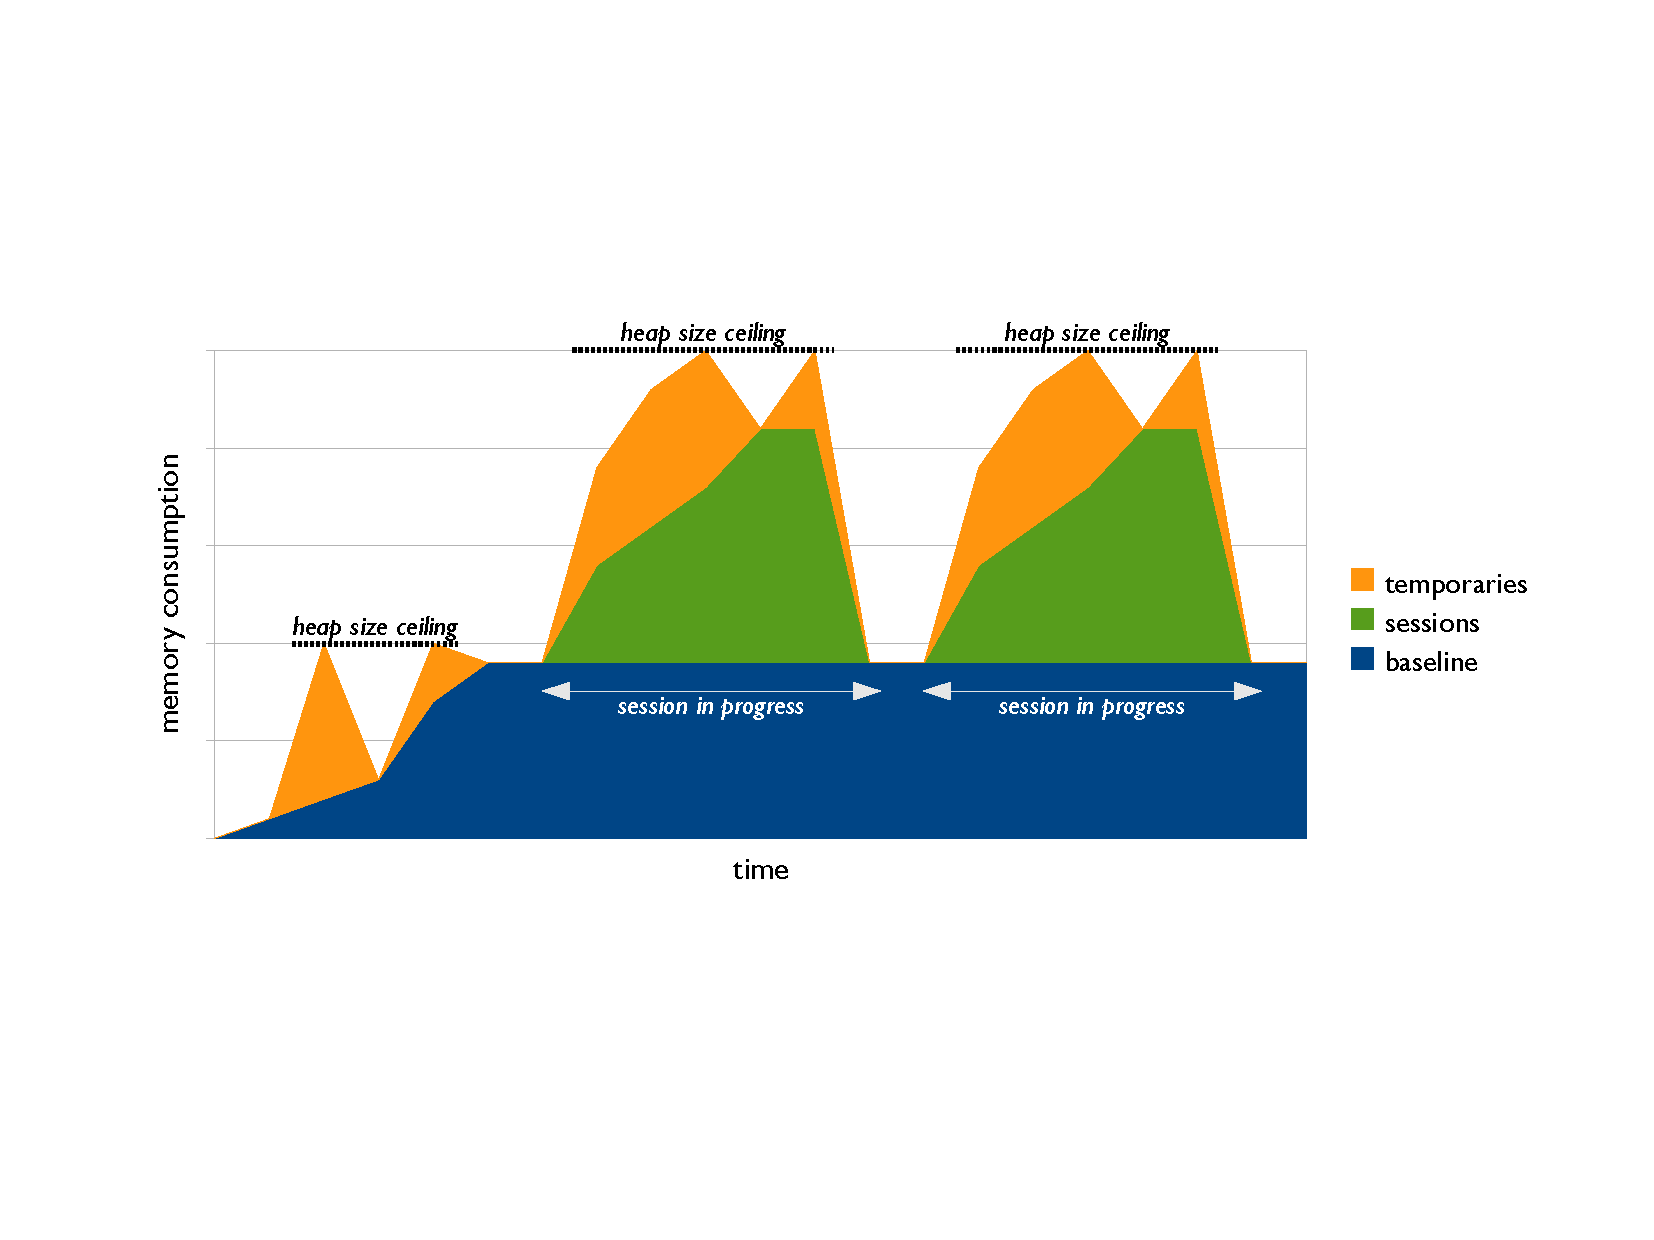
\includegraphics[width=\textwidth]{part4/Figures/lifetime/timeline-base-session-temps}
	\caption{Memory consumption, over time, typical of a web application server.}
	\label{fig:timeline-base-session-temps}
\end{figure}

The heap consumption of this application will fluctuate over time. A timeline
view expected memory consumption helps to illustrate the five main kinds of
object lifetime. It visualizes memory during the lulls and peaks of activity, as
requests are processed and when sessions time out, and as the server starts up.
 \autoref{fig:timeline-base-session-temps} shows an example timeline
for a server that, as it starts up begins to load catalog data into the Java heap.
Then, it responds to one request at a time. The total height of the area under
the curves represents the memory consumption at that point in time. 
In this example, as the server starts up, it begins to load catalog data into
the heap. This data will be used for the entire duration of the server process.
\index{Objects That Live Forever}
The Java objects that represent this catalog are objects that are needed
forever. In the timeline picture, this data is respresented by the lowest area,
labeled \emph{baseline}. Notice how it ramps up quickly, and then, after the
server has reached a ``warmed up'' state, memory consumption of this baseline
data evens out on a plateau for the remainder of the run.

\index{Session State}
After the server is warmed up, it begins to process client requests. Imagine
interacting with a commerce site. First you browse around for items of
interest. You may add items to your shopping cart. Eventually, you may
authenticate and complete a purchase. 
As you browse and buy, the server may be maintaining some
state, to remember aspects of what you have done so far. This
session state, at least the part of it stored in the Java heap, will go away
soon after your browsing session is complete. In the timeline figure, this
portion of memory is labeled \emph{sessions}. It ramps up while a session is in
progress, and then, in the example illustrated here, soon all of that session
memory should be reclaimed.

The catalog (baseline) data and session state are both examples of objects that
are expected to stick around for a while.
\index{Temporary Objects}
 In the course of preloading the cache
and responding to client requests, the server application will create a number
of objects that are only used for a very short period of time. They help to
faciliate the main operations of the server.
These temporary objects will be reclaimed by the \jres garbage collector in
relatively short order. The point at which an object is reclaimed depends on when the garbage collector
notices that it is reclaimable. Normally, the garbage collector will wait until
the heap is full, and then inspect the heap for the objects that are still
possibly in use. In this way, the area under the \emph{temporaries} curve has a
see-saw shape. As the temporaries pile up, waiting for the next garbage
collection, they contribute more and more to memory footprint. Normally, once
the \jre runs a garbage collection, these temporaries no longer in use will no
longer contribute to heap consumption.

In this way, temporary objects
\emph{fill up the headroom} in the heap.\index{Heap Headroom}. If there is a
large amount of heap space unused by the longer-lived objects, then the
temporaries can be reclaimed less often. This is a good thing, because a
garbage collection is an expensive proposition.
\index{Heap Size Settings} \index{Maximum Heap Size} \index{-Xmx}
When configuring your application, you may specify a maximum heap size. It
should certainly be larger than the baseline and session data. How much
larger than that? This choice directly affects the amount of \emph{headroom},
 that is the amount of space available for temporaries to pile up.

\begin{figure}
	\centering
	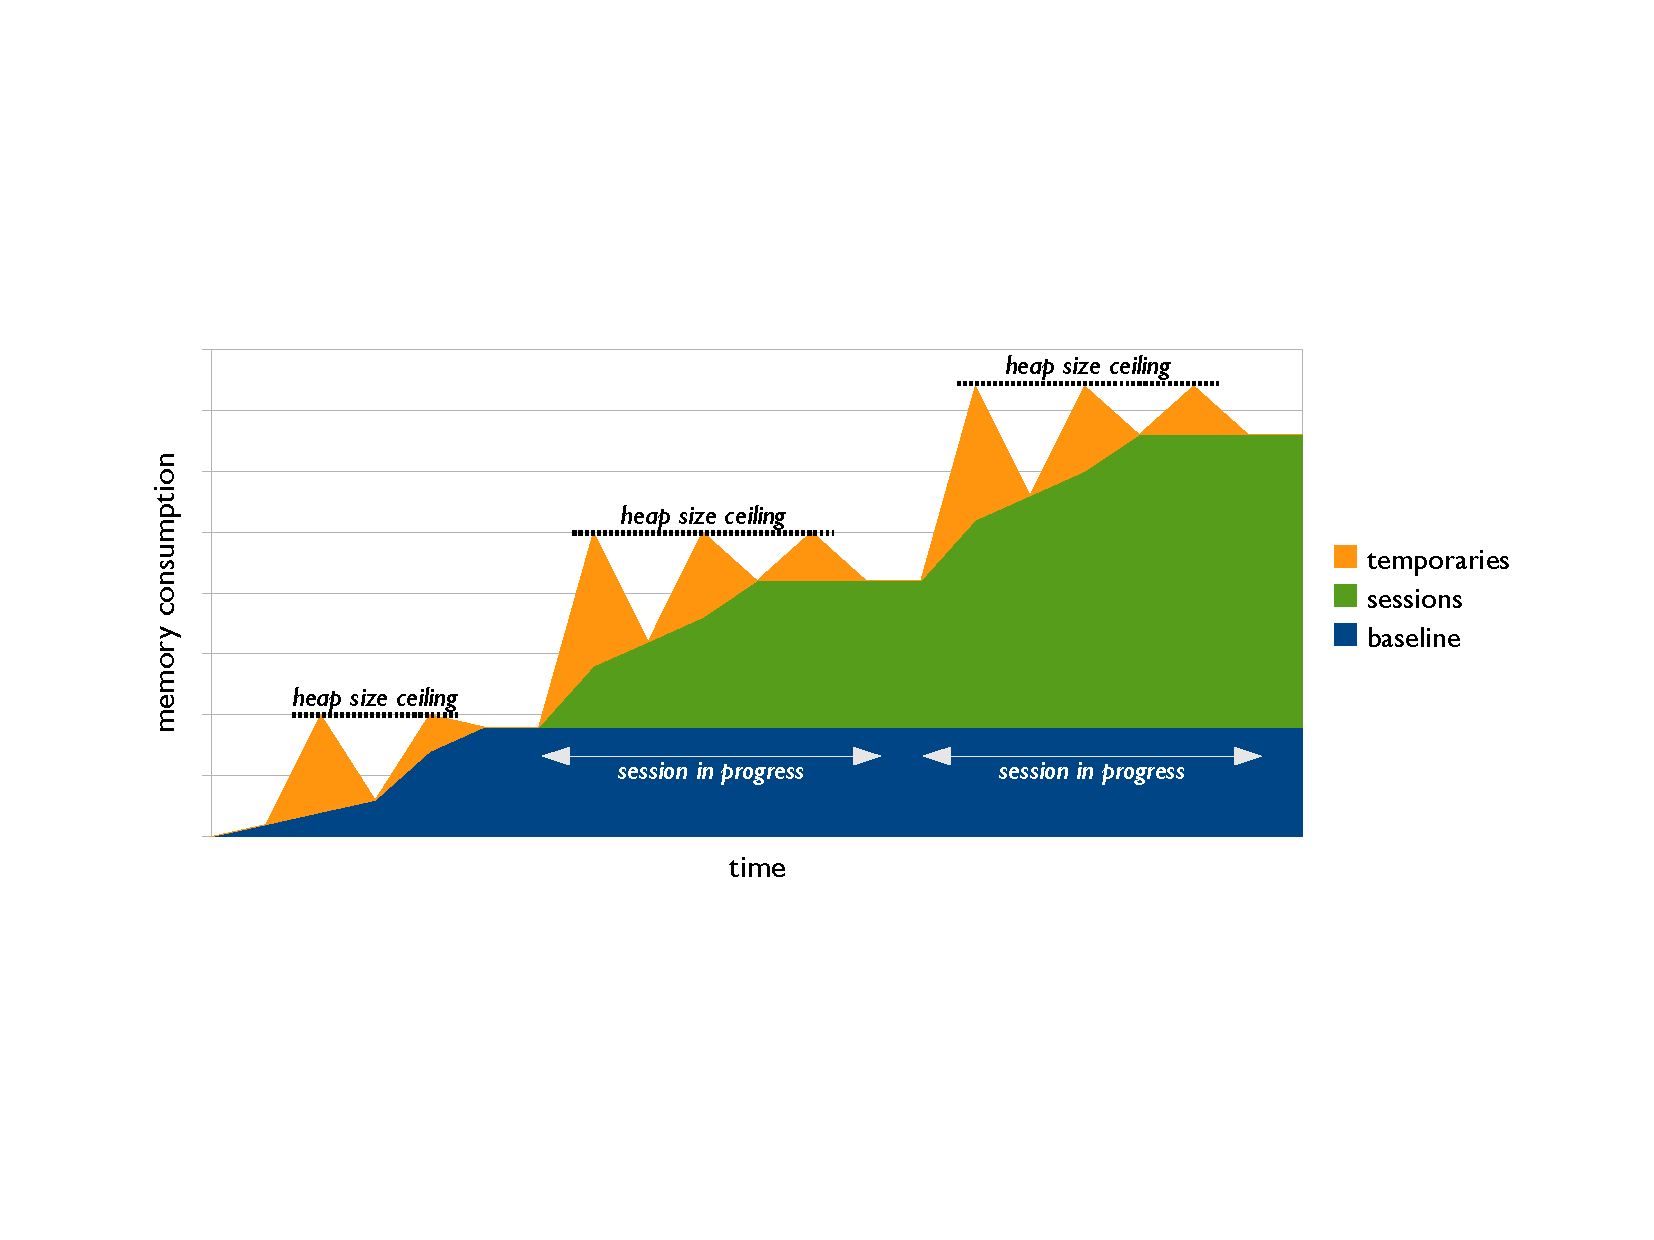
\includegraphics[width=\textwidth]{part4/Figures/lifetime/timeline-base-session-temps-with-leak}
	\caption{If session state is not cleaned up
	properly, a memory leak is the result. This means more frequent garbage
	collections, and ever increasing heap size.}
	\label{fig:timeline-base-session-temps-with-leak}
\end{figure}

\index{Memory Leaks}
The catalog data should last forever, while the
session data lives for some bounded period of time. It is possible that session
state will live beyond the end of your session, but nonetheless it has a
lifetime that is bounded. If, due to an bug, part of this session state is not
reclaimed, the application will leak memory. Though it is supposed to have a bounded lifetime, it
\marginpar{\textbf{Memory Leaks} are still possible, even with
automatic garbage collection!} accidentally lives forever. In this
case, over time, the amount of heap required for the application to run will increase without bound.
\autoref{fig:timeline-base-session-temps-with-leak} illustrates this situation,
in the extreme case when all of session state leaks. Over time, the area under
the curve steps higher and higher.

%As you scan the timeline from left to right, memory consumption 
%it fetches catalog data from its database, and stores them in the Java heap. 

Finally, this example server caches data from some expensive third-party data
source. When caching data inside of Java objects, there is a fourth effect on
the timeline landscape. The
cached data must be configured properly to live long enough to be useful. It
also must not occupy so much of the heap so as to leave little headroom for
temporaries. \autoref{fig:timeline-base-session-temps-with-cache} shows an
example where the cache has probably been configured to occupy too much heap
space. Observe how, compared to the other timeline figures, there is little
headroom for temporaries. In this case, the result is more frequent garbage
collections. If the cache were sized to occupy an even greater amount of heap
space, it is possible that there would no longer be room to fit session data.
The result in this case would be failures in client requests. So, as you can
see, sizing caches is important. As discussed later, it is very tricky to
properly size caches, and is something best left in the hands of the \jre.

\begin{figure}
	\centering
	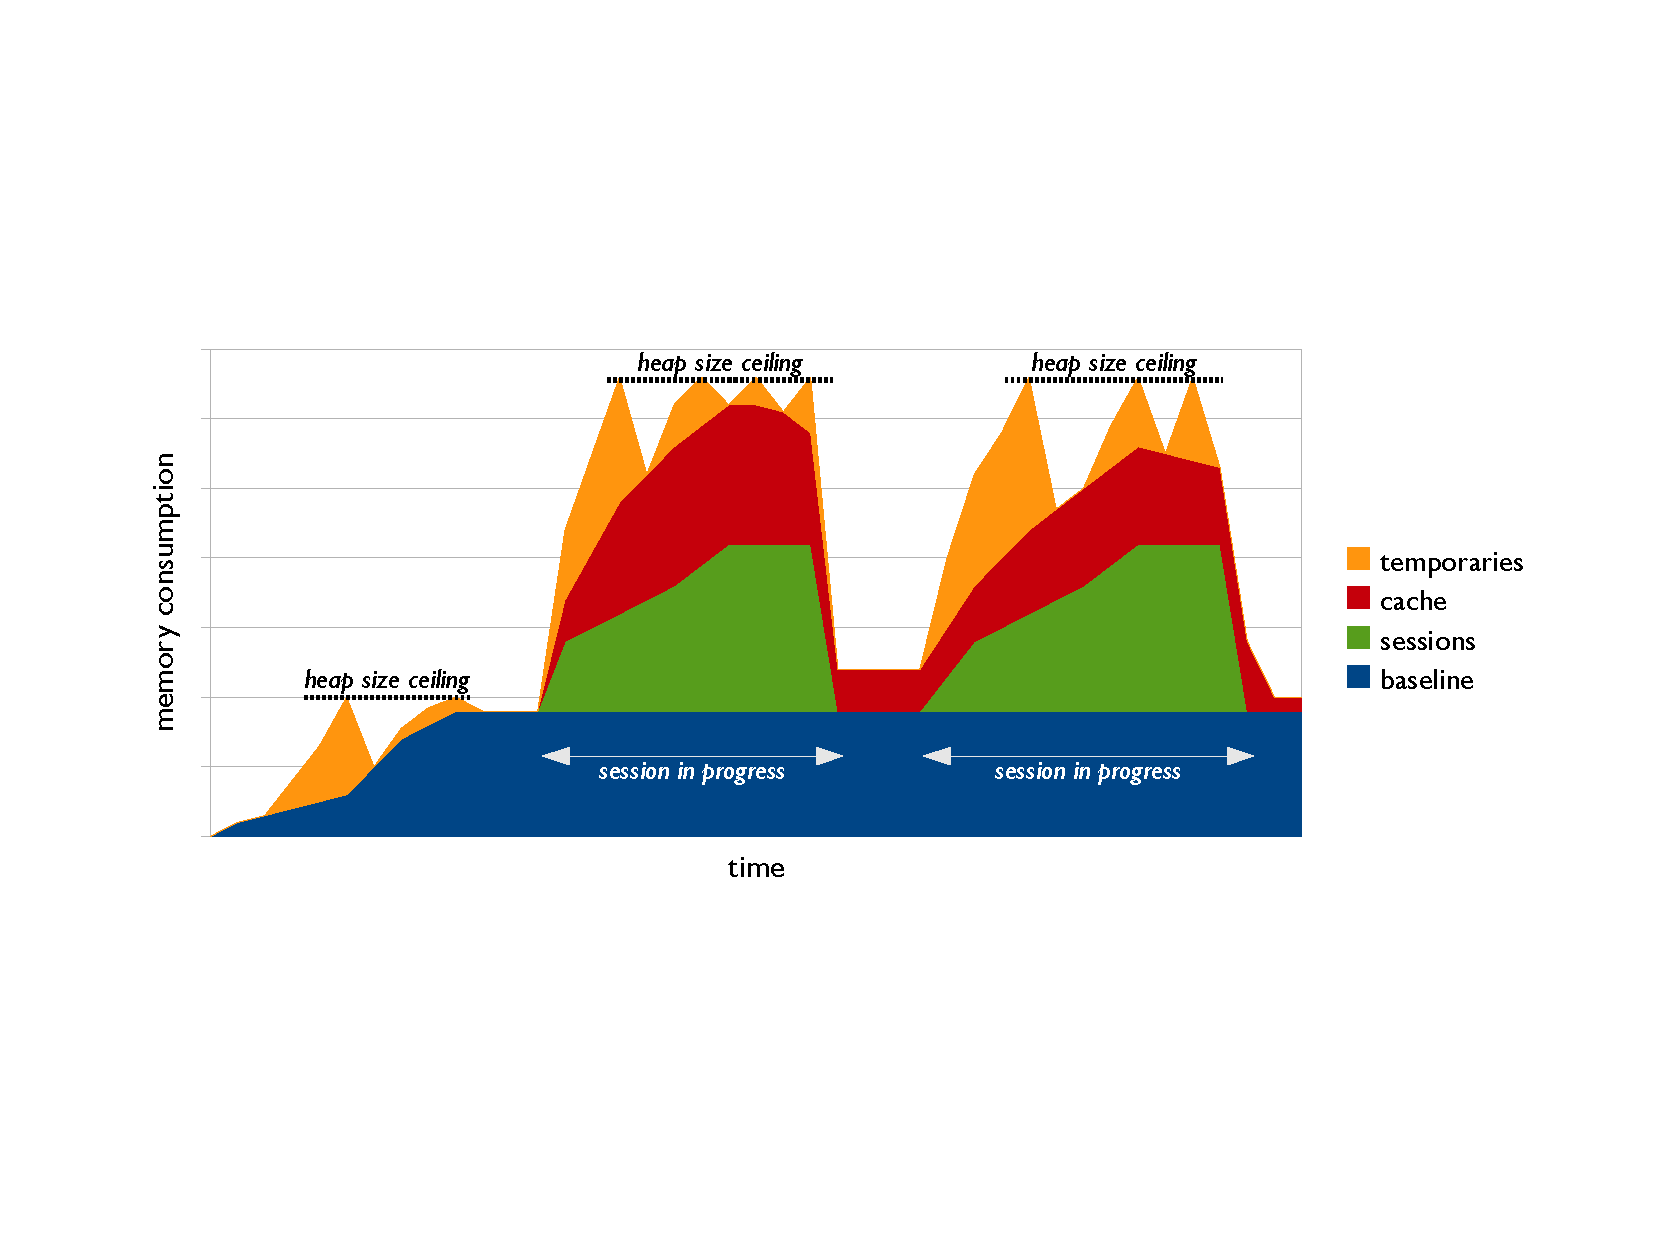
\includegraphics[width=\textwidth]{part4/Figures/lifetime/timeline-base-session-temps-with-cache}
	\caption{When a cache is in use, this leaves less headroom for temporary
	object allocation, often resulting in more frequent garbage collections.}
	\label{fig:timeline-base-session-temps-with-cache}
\end{figure}

% introduced by example in this chapter, and
%Many objects are either temporaries or needed for
%the entire run of your application. Sometimes you create objects whose lifetime
%is correlated with other objects or that should go away when a method
%invocation completes. Sometimes you need to manage objects hanging around
%longer than their current need, to avoid future recomputations or refetching
%of data in the case when it is needed in the near future. 

%\begin{table}
%\centering
	%\begin{tabular}{ll} \toprule
    %%%%	%& Things Java Doesn't Do Automatically \\ \cmidrule{2-2}
%    	\autoref{avoiding-lifetime-bugs} & {Avoiding Memory Leaks} \\
%    	\autoref{balance-time-and-space} & {Balancing Time and Space} \\
%    	\autoref{outisde-java-box} & {Supporting Massive Data Sets}  	\\
%        \bottomrule
%    \end{tabular}
%	\caption{The tricky aspects of memory management.}
%	\label{tab:tricky-memory-management}
%\end{table}

\section{Temporary Objects}
\label{temporary-lifetime}

If your application is like most Java applications, it creates a large number of
temporary objects. They hold data that will only be used for a very short
interval of time. It is often the case that the objects in these transient data
structures are only ever referenced by local variables. For example, this is the
case when you populate a \class{StringBuffer}, turn it into a \class{String}, and
then ultimately (and only) print the string to a log file. The point at which all
of these objects, the strings and character arrays, are no longer used is only
shortly after they are constructed. These objects serve as transient homes for
your data, as it makes its way through the frameworks and libraries you depend
on. Temporaries are often necessary to bridge separately developed code and
enable code reuse: as long as you can convert your data layout into a form that
an API requires, then you can reuse the functionality it provides.

In many cases, you need do nothing special to manage the temporary objects your
application creates. After all, generational garbage collectors these days do a
very good job digesting a large volume of temporary objects. In a generational
garbage collector, the \jre places temporary objects in a separate heap, and
thus it need only process the newly created objects during its routine scan.

Unfortunately, in Java it is pretty easy to create a high volume of temporary
objects. Say your application 
fills up the temporary heap ever second. In this case, based on the common
speeds of garbage collectors, your application could easily spend over 20\% of its time
collecting garbage.
Is it difficult to fill up the temporary heap once per second? Typical
temporary heap sizes run around 128 megabytes. Say your application is a serves
a peak of 1000 requests per second, and creates objects of around 50 bytes each.
If it creates around 2500 temporaries per request, then this application will
spend 20\% of its time collecting garbage.


%A great many of these
%temporary structures serve the role of a kind of lubricant, making it easy for
%you to write code that ties together the separately written parts of your code
%base and reuses standard libraries as much as possible. Often, these are
%objects that are not a fundamental necessity of what you're trying to
%accomplish. If
%you had the freedom to code highly specialized implementations of the important
%cases, from scratch, many of these temporary structures would be unnecessary.

\begin{example}{How Easy it is to Create Lots of Temporary Objects}
A common example of temporaries is parsing
and manipulating data coming from the outside world. Identify the temporary
objects in the following code.
% to the wire?

\begin{shortlisting}%[float,caption=Code that constructs 8 temporary objects tohandle two dates.,label=TempExampleCode]
void main(String xy) {
	doWork(xy.substring(0,10), xy.substring(10));
}	
void doWork(String x, String y) {
	doRemoveProcedureCall(parse(x));
	doRemoveProcedureCall(parse(y));
}
Date parse(String string) {
	return new SimpleDataFormat().parse(string, new ParsePosition(0));
}
void doRemoteProcedureCall(Date date) {
	long timestamp = date.getTime();
	...
}
\end{shortlisting}
\end{example} 

This code starts in the \code{main} method by splitting the input string into two
substrings. So far, the code has created four objects (one \class{String} and one
character array per substring). Creating these substrings makes it easy to use
the \code{doWork} method, which takes two Strings as input. However, observe that
these four objects are not a necessary part of the computation. Indeed, these
substrings are eventually used only as input to the \class{SimpleDateFormat}
\code{parse} method, which has been nicely designed to allow you to avoid this
very problem. By passing a \class{ParsePosition}, one can parse substrings of a
string without having to create temporary strings (at the expense of creating
temporary \class{ParsePosition} objects!).



% correlated with need: as soon as last user goes away, remove his stuff 
% share common expressions to save space, but using strong references -> memory
% leak; plugins in eclipse go away when all views
% sharing pool 

% weak ref keys -> annotation
% weak ref values -> sharing pool

% soft ref values -> caching

% annotation by map lookup


\section{Objects Needed Forever}
\label{forever-lifetime}

A \class{SimpleDateFormat} object in the previous example was created in every
loop iteration, and never used again. An improvement would be to create and
use a single formatter for the remaining duration of the run. Though the Java 6
documentation does not say so explicitly, it is safe to reuse a single instance
of this object multiple times. You must be careful to remember that it is
not safe to do so in multiple threads. The next chapter will discuss remedies
to this problem. The updated code for the \code{parse} method would be:

\begin{shortlisting}
static final DateFormat fmt = new SimpleDateFormat();

Date parse(String string) {
	return fmt.parse(string, new ParsePosition(0));
}
\end{shortlisting} 

A \code{static} field of an object is one way that Java gives you to indicate
that you want an object to live forever.

\section{Objects with Correlated Lifetimes}

Many objects are needed for a very specific interval of time. This interval is
usually defined either by the lifetime of another object, or by the duration of
a method call. Once that other object is not needed, or once that method
returns, then these objects are also no longer needed. These are the two many
cases of objects with correlated lifetime.

\subsection{Objects that Live and Die Together}
\label{correlated-lifetime-1}

Normally, if you need to augment the state stored an object, you modify
the source code of some existing classes. For example, to add a secondary
mailing address to a \class{Person} object, you can add a field to that class, and update the
initialization and marshalling logic accordingly. Sometimes, you will find it
necessary to associate information with an object that is, for one reason or the
other, locked down.

\begin{example}{Annotations}
In order to debug a performance problem, you need to associate a timestamp with
another object. Unfortunately, you don't have access to the source code for
that object's class. Where do you keep the new information, and how can you
link the associated storage to the main objects without introducing memory
leaks?\index{Memory Leaks}
\end{example}

If you can't modify the class definition for that object, then you will have to
store the extra information elsewhere. These \emph{side annotations}\index{Side
Annotations} will be objects themselves, and you need to make sure that their
lifetimes are correlated with the main objects. When one dies, the other
should, too.

You could store the annotations in a map that is keyed by the
original object, say of type \class{T}:

\begin{shortlisting}
Map<T, Date> timestamps = new HashMap<T, Date>();

void addTimestamp(T t) {
	timestamps.put(t, new Date());
}
Date getTimestamp(T t) {
	return timestamps.get(t);
}
\end{shortlisting}

This solution will function correctly, but suffers from a \emph{memory
leak}\index{Memory Leak}. As the application runs, it will consume greater
amounts of Java heap, up until the point when the \jre runs out of heap space to
allocate any more objects. This solution leaks memory, because the
\code{timestamps} map introduces a reference to the main objects. When the
garbage collector scans the heap to see which objects are still alive, the
references in this map will be among those that keep the objects alive. The next
chapter discusses these issues in more detail. An improved solution would use the
\class{WeakHashMap} from the Java standard libraries. By replacing the
initialization of the \code{timestamps} map, we have the same functionality as
before, but no memory leak.

\begin{shortlisting}
Map<T, Date> timestamps = new WeakHashMap<T, Date>();
\end{shortlisting}

Note that this same situation can hold even if you are able to modify the class
definition. A common scenario requires annotations on only a subset of all
instances of a class. In this case, is it not worth paying the memory cost to
have the ability to annotate every single instance. Therefore, this is another
case where a solution of side annotations, stored in a \class{WeakHashMap},
shines.

\subsection{Objects that Live and Die with Program Phases}
\label{correlated-lifetime-2}

Similar to the way the lifetime of an object can be correlated with another
object, lifetimes are often correlated with method invocations. When a method
returns, objects correlated with it should go away. For temporary objects, this
is usually easy to ensure, since they are usually only referenced by stack
locations. For the medium-to-long running methods that implement the
core functionalities of the program, this correlation is harder to get right.

For example, if your application loads a log file from disk,
parses it, and then displays the results to the user, it has roughly three
phases for this activity. Most of the objects allocated in one phase are scoped to that
phase; they are needed to implement the logic of that phase, but not subsequent
phases. The phase that loads the log file is likely to maintain maps that
help to cross reference different parts of the log file. These are necessary
to facilitate parsing, but, once the log file has been loaded, these maps can be
discarded. In this way, these maps live and die with the first phase of this
example program. If they don't, because the machinery you have set up to
govern their lifetimes has bugs, then your application has a memory
leak\index{Memory Leaks}.

This lifetime scenario is also common if your application is an
server that handles web requests.

\begin{example}{Memory Leaks in an Application Server}
	A web application server handles servlet requests. How is it possible that
	objects allocated in one request would unintentionally survive beyond the end
	of the request?
\end{example} 
  
In server applications, most
objects created within the scope of a request should not survive the
request. Most of these \emph{request-scoped}
\index{Request-scoped Lifetime} objects are not used by the application after the
request has completed. In the absence of application or framework bugs, they will
be collected as soon as is convenient for the runtime. In this example, the
lifetime of objects during a request are \emph{correlated} with a method
invocation: when the servlet \class{doGet} or \class{doPut} (etc.) invocations
return, those correlated objects had better be garbage collectible.

\index{Memory Leaks: Why?}
There are many program bugs and configuration missteps that can lead to
problems. The general problem is that a reference to an object stays around
indefinitely, but becomes
\emph{forgotten}, and hence rendered unfindable by the normal application
logic. If this request-scoped data structure were only reachable from stack
locations, you would be fine. Therefore, a request-scoped object will leak only
when there exist references from some data structure that lives forever. Here
are some common ways that this happens.

\begin{itemize}
  \item Registrars, where objects are registered as listeners to some service,
  but not deregistered at the end of a request.
  \item Doubly-indexed registrars. Here the outer map provides a key to index
  into the inner map. A leak occurs when the outer key is mistakenly
  overwritten mid-request. This can happen if the namespace of keys isn't
  canonical and two development groups use keys that collide. It can also
  happen if there is a mistaken notion, between two development groups, of who
  owns respnsibility of populating this registrar.
  \item Misimplemented hashcode or equals, which foils the retrieval of an
  object from a hash-based collection. If developers checked the return value of
  the \code{remove} method, which for the standard collections would indicate a failure to remove, then
  this bug could be easily detected early; but developers tend not to do this.
\end{itemize}

The next chapter goes into greater detail on how to avoid these kinds of
errors. \autoref{chapter:tools} describes tooling that can help you
detect and fix the bugs that make it into your finished application.


%\subsection{Correlated with Need} % do we need this? isn't session state a
% deferred deletion policy?
%\label{correlated-lifetime-3}

\section{Objects with Deferred Deletion}
\label{deferred-deletion}

The last important facet of object lifetime comes from those objects that stay
around beyond the scope of any one method or object. These objects must survive
for some indeterminant amount of time. In some cases, this period based on the
profitability of keeping them around. In other cases, objects need to be kept
around for operations that span several independent operations across multiple
threads.
There are three important cases of objects that need to be reclaimed in some
deferred fashion: caches, sharing pools, and resource pools.

\subsection{Caches: Buying Time with Space}
\label{sec:caches}
\index{Caches}

\marginpar{A \textbf{Cache} is a map that holds expensive data values, each
accessed by a unique key.}
If the data stored in an object is cheap to recompute or refetch from an
external data source, then a good policy would be to treat the object as a
temporary. Performing a few dozen machine instructions is very likely to be a
worthwhile trade-off, if memory consumption is the limiting resource for
scaling up\index{Scaling Up}. 
You do have to be careful, though. Recall our earlier example that creates a new
instance of the date parser \class{SimpleDateFormat} for each iteration of a
loop. Here, as is quite common, something expensive to compute, that
\class{SimpleDateFormat}, is treated as a temporary. If the data stored in an
object is expensive to recompute or refetch, and there is some chance it might
be used in the future, then it is worthwhile to keep it around.

\index{Time-Space Trade-offs}
Finding the right balance of time and space is the goal of a good cache
implementation. The expense of re-fetching data from external data sources and
recomputing the in-memory structure can often be amortized, at the expense of
stretching the lifetime of these data structures. By increasing the actual
lifetime on an object you will very likely increase peak memory consumption. A
good cache defers the time that an object will be reclaimed, as long as there is
sufficient space to handle the flux of temporary objects your application
creates. It holds on to a data structure after the current operation is finished
with it, in the hope that other operations in the near future will reuse it.

\subsection{Sharing Pools: Avoiding Data Replication}
\label{sec:sharing-pools}
\index{Sharing Pool}

\marginpar{A \textbf{Sharing Pool} stores canonical instances of data
values that would otherwise be replicated in many objects.}
A cache amortizes the time cost of fetching or initializing data. An orthogonal
issue lies in the memory expense of storing many copies of the same data
throughout the heap. This is especially a problem with strings. Heaps can often
store the same string a dozen times.

\begin{example}{Duplicate Strings}
You application loads data from a file. This data contains a large number of
name-value maps that will be used frequently throughout program execution.
These maps represent configuration information. The names come from a small set
of 16 distinct names. The values are strings come from
a set of strings unknown at development time, but a set that is small in size;
there aren't going to be many distinct values, but you are unwilling or unable
to nail them down at compile time. How can these maps be stored in a memory
efficient way?
\end{example}

Without any special effort, each instance of this kind of configuration map
would store the some subset of same 16 key strings. Furthermore, each map would
store duplicates of the values. The following code snippet has those two
aspects of duplication:

\begin{shortlisting}
void handleNextEntry() {
	String key = getNextString();
	Object value = getNextString();
	map.put(key, value);
}
\end{shortlisting} 

Java provides a built-in mechanism for sharing the contents of strings across
many string instances. By \emph{interning}\index{String interning} a Java
\class{String}, you ensure that the returned \class{String} will only have
distinct storage if it is a string value that hasn't been interned yet. You can
modify the first try as follows:

\begin{shortlisting}
void handleNextEntry() {
	String key = getNextString().intern();
	Object value = getNextString().intern();
	map.put(key, value);
}
\end{shortlisting} 

It is possible to do even better, if you have the luxury of modifying both ends
of the communication channel, i.e. both the serialization and this
deserialization code. There are only 16 distinct names used in all instances of
this configuration map. This seems like a perfect case for an enumerated type.
An enumerated type can be used to represent strings as numbers at runtime. The
only place the strings are stored is in the string constant pool\index{Java's
Constant Pools}. Each class, when compiled, keeps a pool of the strings that
are used by code in that class. In this way, an enumerated type is an even more
highly optimized sharing pool than that provided by the interning mechanism:

\begin{shortlisting}
enum PropertyName = {...};
void handleNextEntry() {
	PropertyName key = getNextPropertyName();
	Object value = getNextString().intern();
	map.put(key, value);
}
\end{shortlisting} 



There is an important variant of a sharing pool called the Bulk Sharing Pool.
Like a normal sharing pool, the goal of a bulk sharing pool is to amortize the
memor costs of storing data. However, rather than mitigate the costs of data
duplication, a bulk sharing pool aims to amortize the costs of Java object
headers across the elements in a pool. This is a topic that stretches notions of
how to store data beyond the normal Java box, and so will be discussed, along
with many similar matters, in \autoref{chapter:outisde-java-box}.


\begin{table}
	\centering
	\begin{tabular}{rlll} \toprule
            & cache             & sharing pool & resource pool 
    \\ \cmidrule{2-4}
%    What is Saved & alloc. and data init. time & duplicates &
    %alloc. time 
%    \\
    Addressing the Contents     & by key       & by index & by key
    \\
        Elements Interchangeable?   & no    & no    & yes
    \\
    Multiple Users per Element? & yes   & yes   & no
    \\
    Data Persists Across Uses?  & yes   & yes   & no
    \\ \bottomrule
    \end{tabular}
	\caption{Comparing the charaacteristics of three mechanisms for keeping data
	or objects around for indefinite periods of time.}
	\label{tab:three-deferred-deletions}
\end{table}

\subsection{Resource Pools: Amortizing Allocation Costs}
\label{sec:resource-pools}
\index{Resource Pool}

\index{Amortizing Costs}
A cache can amortize the cost, in time, of fetching or otherwise initializing the
data stored in an object. A sharing pool can amortize the cost, in space, of
storing the same data in many separate objects. In both cases, the data is the
important part of what is stored.

\marginpar{A \textbf{Resource Pool} is a set of interchangeable storage or
external connections that are expensive to construct.} There is a third case,
where one needs to amortize the cost of the allocations, rather than the cost of
initializing or fetching the data that is stored in this object. A resource pool
stores the result of the allocation, not the data. Therefore, the elements of a
resource pool are interchangeable, because it is the storage, not the values that
matter. It is important to note that, though the data values are not the
important part, the elements of the pool are objects, and are thus intended to
store data! A resource pool handles the interesting case where the data is
temporary, but you need, for performance reasons, the objects to live across many
uses. The protocol for using a resource pool then involves reservation, a period
of private use of the fields of the reserved object, followed by a return of that
object to the pool.

Resource pooling only makes sense if the allocations themselves are expensive.
There are several reasons why a Java object can be expensive to allocate.
Creating and zeroing a large array\index{Large Arrays} in each iteration of a
loop can bog down performance. Creating a new key object to determine whether an
value exists in a map can sometimes contribute a great deal to the load of
temporary objects.

\index{Connection Pools}
A more important example of the need for amortizing the time cost of allocation
comes when this Java object is a proxy for resources outside of Java. If your
application accesses a relational database through the JDBC\index{JDBC}
interface, you will experience the need for resource pooling. There are two kinds
of objects that serve as proxies for resources involving database access. First
are the connections to the database. In most operating systems, establishing a
network connection is an expensive proposition. It also involves reservation of
resoures in the database process. Second are the precompiled SQL statements that
your application uses. As with the connections, these involve setup cost, of the
compilation itself, as well as the reservation of memory resources, that the
database uses to cache certain information about the query.

\begin{example}{Per-thread Singleton versus Resource Pool}
\index{Thread-Local Storage}
Your application accesses a remote resource. Why not keep one connection
persistent per thread? What's the point of a resource pool in this case?
\end{example}


%% OLD STUFF NMM 20090820
%\section{Request Scoping}
%\section{Correlated Lifetime}
%\paragraph{Weak and Soft references in Java}
%\section{Memory Leaks and Drag}
%\section{Examples}
%\subsection{Transient Near-Copies}
%\subsubsection{String Canonicalization}
%\subsection{Temporary Collections}
%\subsection{Facilitators}

% TODO maybe introduce weaks and softs??

\chapter{Memory Fundamentals}

Before getting into the details of how to implement your lifetime requirements,
it is important to understand some of what the fundamentals of memory management
in languages like Java. The Java language has a \emph{managed runtime}. In part,
this means that, as a Java program runs, a runtime environment assumes the burden
of key aspects of memory management. This level of management includes as
automatic garbage collection of both instances and Java classes. Therefore, Java
has feature that govern, on your behalf, important aspects of the lifetime of
objects. You need to appreciate what the runtime is doing for you, before
considering how to reshape object lifetimes to better suit your needs.

Designing a lifetime management strategy requires that you take the tools that
Java provides, and combine them with other strategies implemented on top of Java.
The built-in mechanisms handle some aspects of the common patterns of object
lifetime. Unfortunately, they often appear in the form of low-level JVM hooks,
and so require careful coding to make correct use of them.

This chapter introduces the basics of the garbage collector, and how the Java
managed runtime governs object lifetimes. Then, it walks you through the
lifecycle of typical objects from allocation to eventual garbage collection. If
you are comfortable with the basics of memory management, you may discover that
you can skip to the next chapter.

\section{The Garbage Collector}
The \jre decides when the storage allocated to an object should be reclaimed.
This decision is based on a number of criteria. The point of reclamation
depends on the settings you have chosen for various policy knobs, and is also
affected by choices you have made in the application code. However, in most
cases, there is a common structure to the schedule of when objects are
collected.

\paragraph{The Collection Schedule}
Most contemporary garbage collectors deallocate storage in a series of bulk
steps. In almost all \jres, memory is not reclaimed one object at a time.
Instead, to amortize the costs involved in reclamation, the garbage collector
often lets reclaimable objects pile up for a while. It then collects then en
masse. As objects are allocated, memory consumption can be observed to increase,
up until some maximum allowed amount. At this point, the collector reclaims
unused memory, and the process starts again. In this way, memory consumption over
time often assumes a sawtooth edge, such as those shown in
\autoref{fig:timeline-base-session-temps-with-cache}.
\index{Sawtooth Pattern}

\paragraph{Configuration Settings}
You can guide the frequency of collection, which will change the slope of this
sawtooth curve to be either more or less jagged. In one common case, the garbage
collector will wait until all available memory is consumed before reclaiming
storage.  In Java, you can configure this ceiling by supplying a sizing to the
\code{-Xms} (initial ceiling) and
\code{-Xmx} (maximum ceiling) command line options. \index{-Xms command line setting}
\index{-Xmx command line setting} The \jre will begin with a ceiling at the
former level. If collections are occuring too frequently, the \jre may decide to
increase the \emph{current} ceiling to a higher level. As the need for memory
fluctuates, so the \jre will raise or lower the current ceiling level. The
current ceiling will always be some value lower than the maximum, \code{-Xmx},
setting. One such scenario, of increasing ceiling level, is illustrated in
\autoref{fig:timeline-base-session-temps-with-leak}.


\paragraph{What a Collection Collects}

\paragraph{The Nursery, Permspace, and Constant Pools}
\index{Nursery}
\index{Permspace}

\paragraph{Finalization and Phantom Referenes}
\index{Finalization of objects}
\index{Phantom References}

\paragraph{Class Unloading and Lifetime of Statics}

A \code{static} field of an object is one way that Java gives you to indicate
that you want an object to live forever.
\index{Class Unloading}
\index{Static fields}

\paragraph{Concurrent, Parallel, and Real-time Collection}
\index{Concurrent GC}
\index{Parallel GC}
\index{Real-time GC}


\section{The Object Lifecycle}
%Every object created by your application lives for an interval of time from its
%creation to the point that the Java runtime gets around to collecting it. An object's {\em natural} lifetime is defined by the
%interval of time between its first and last necessary use. %cite drag paper
%here?


In a \emph{well-behaved} application, an object's lifetime spans its allocation,
use, and the short period during which the \jre takes control and reclaims the
space. For some subset of an object's actual lifetime, that is the time from
creation to reclamation, your application will make use of the data stored in its
fields. \autoref{fig:typical-lifecycle} illustrates the lifecycle of a typical
object in a well behaved application.

\begin{figure}
	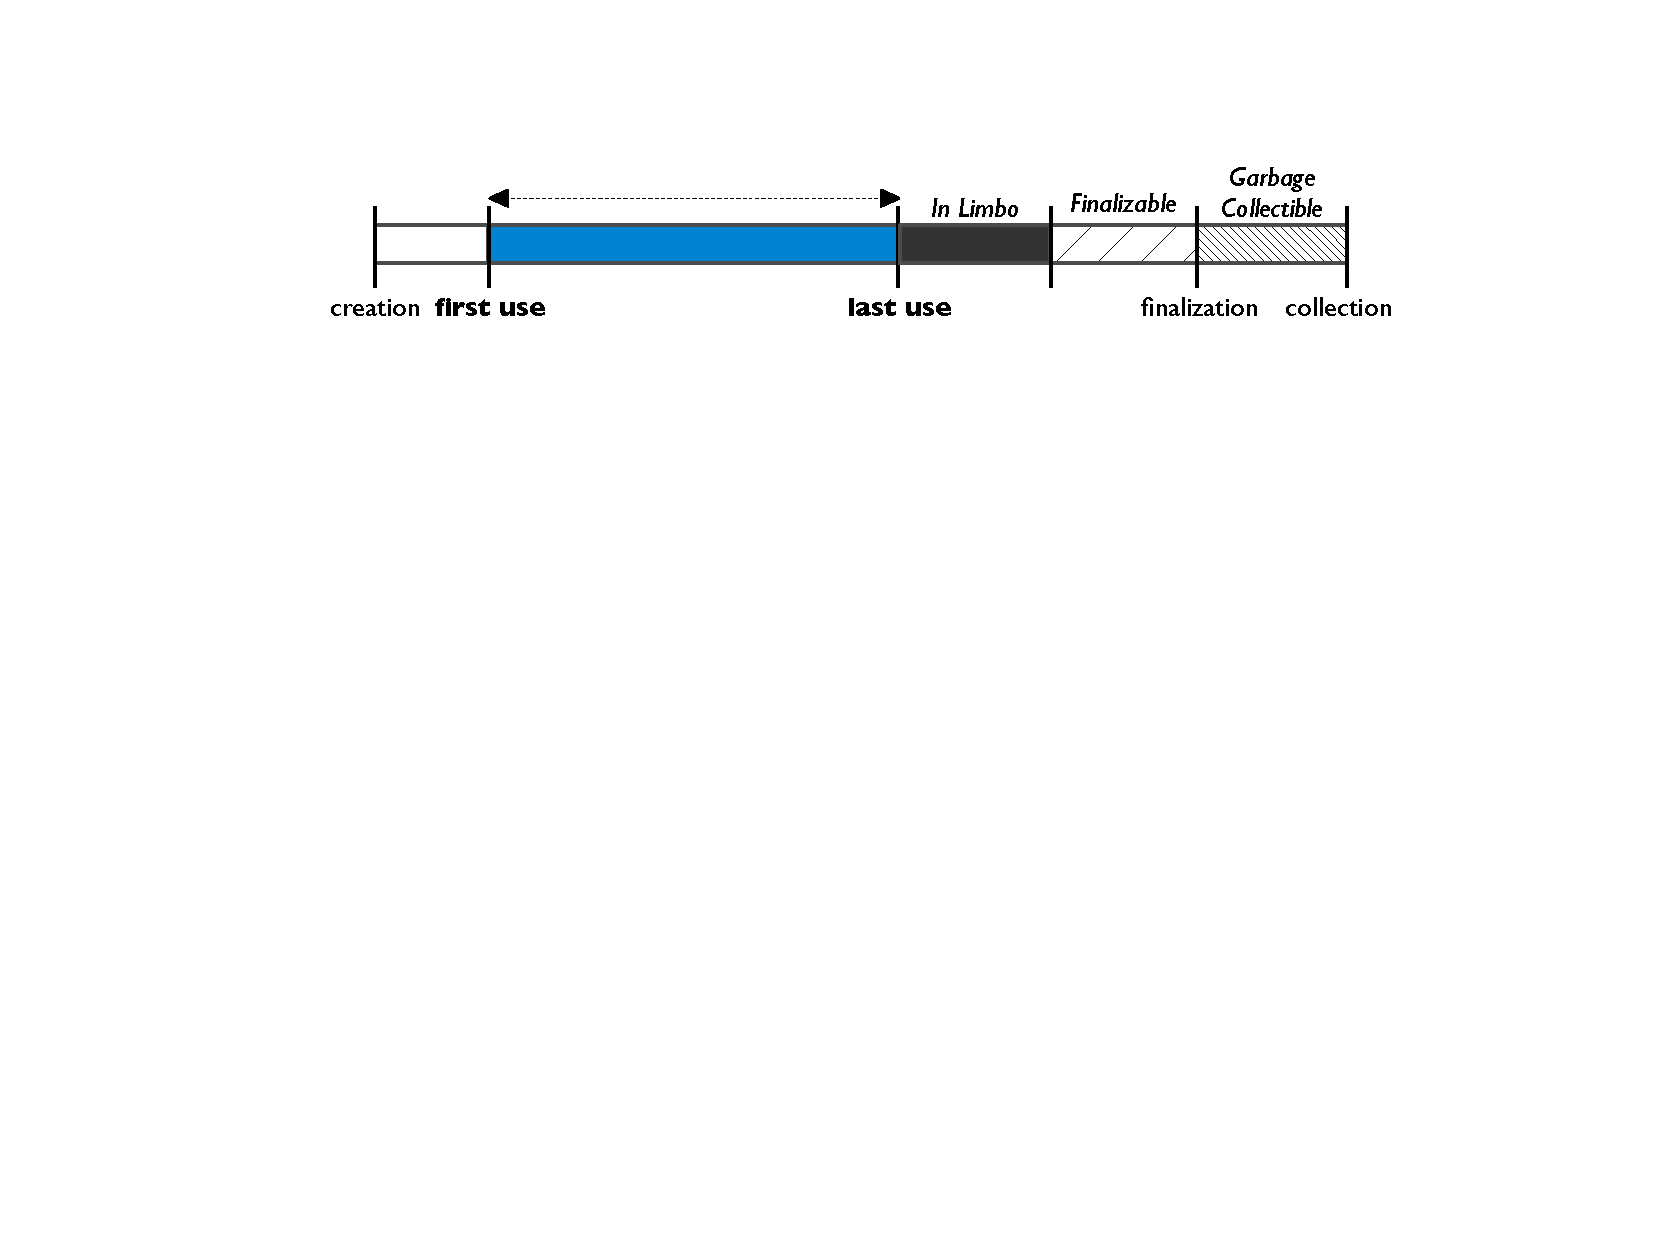
\includegraphics[width=0.9\textwidth]{part4/Figures/lifetime/object-lifecycle}
	\caption{Timeline of the life of an object.}
	\label{fig:typical-lifecycle}
\end{figure}

\begin{example}{Parsing a Date} Consider a loop that shows an easy way to parse
a list of dates. What objects are created, and what are their lifetimes?
\begin{shortlisting}
for (String string : inputList) {
	ParsePosition pos = new ParsePosition(0);
	SimpleDateFormat parser = new SimpleDateFormat();
	System.out.println(parser.parse(string, pos));
}
\end{shortlisting}
\end{example}

For each iteration of this loop, this code takes a date that is represented as a
string and produces a standard Java \class{Date} object. In doing so, a number of
objects are created. Two of these are easy to see, in the two \code{new} calls
that create the parse position and date parser objects. The programmer who wrote
this created two objects, but many more are created by the standard libraries to
finish the task. These include a calendar object, number of arrays, and the
\class{Date} itself. None of these objects are used beyond the iteration of the
loop in which they were created. Within one iteration, they are created, almost
immediately used, and then enter a state of \emph{limbo}.

\callout{limbo}{Objects in Limbo}{
\index{Limbo}
In limbo, an object will never be used again, or at least not for long time,
but the \jre doesn't yet know that this is the case. The object hangs
around, taking up space in the Java heap until the point when it exits limbo.}

The \code{pos} object represents to the parser the position within the
input string to begin parsing. The implementation of the \code{parse} method
uses it early on in the process of parsing. Despite being unused for the
remainder of the parsing, the \jre does not know this until the current
iteration of the loop has finished. This time in limbo also includes the
entirety of the call to \code{System.out.println}, an operation entirely
unrelated to the creation or use of the parse position object. Once the current
loop iteration finishes, these two objects will exit limbo, and become garbage
collectible.\index{Exiting Limbo}

\begin{figure}
	\centering
	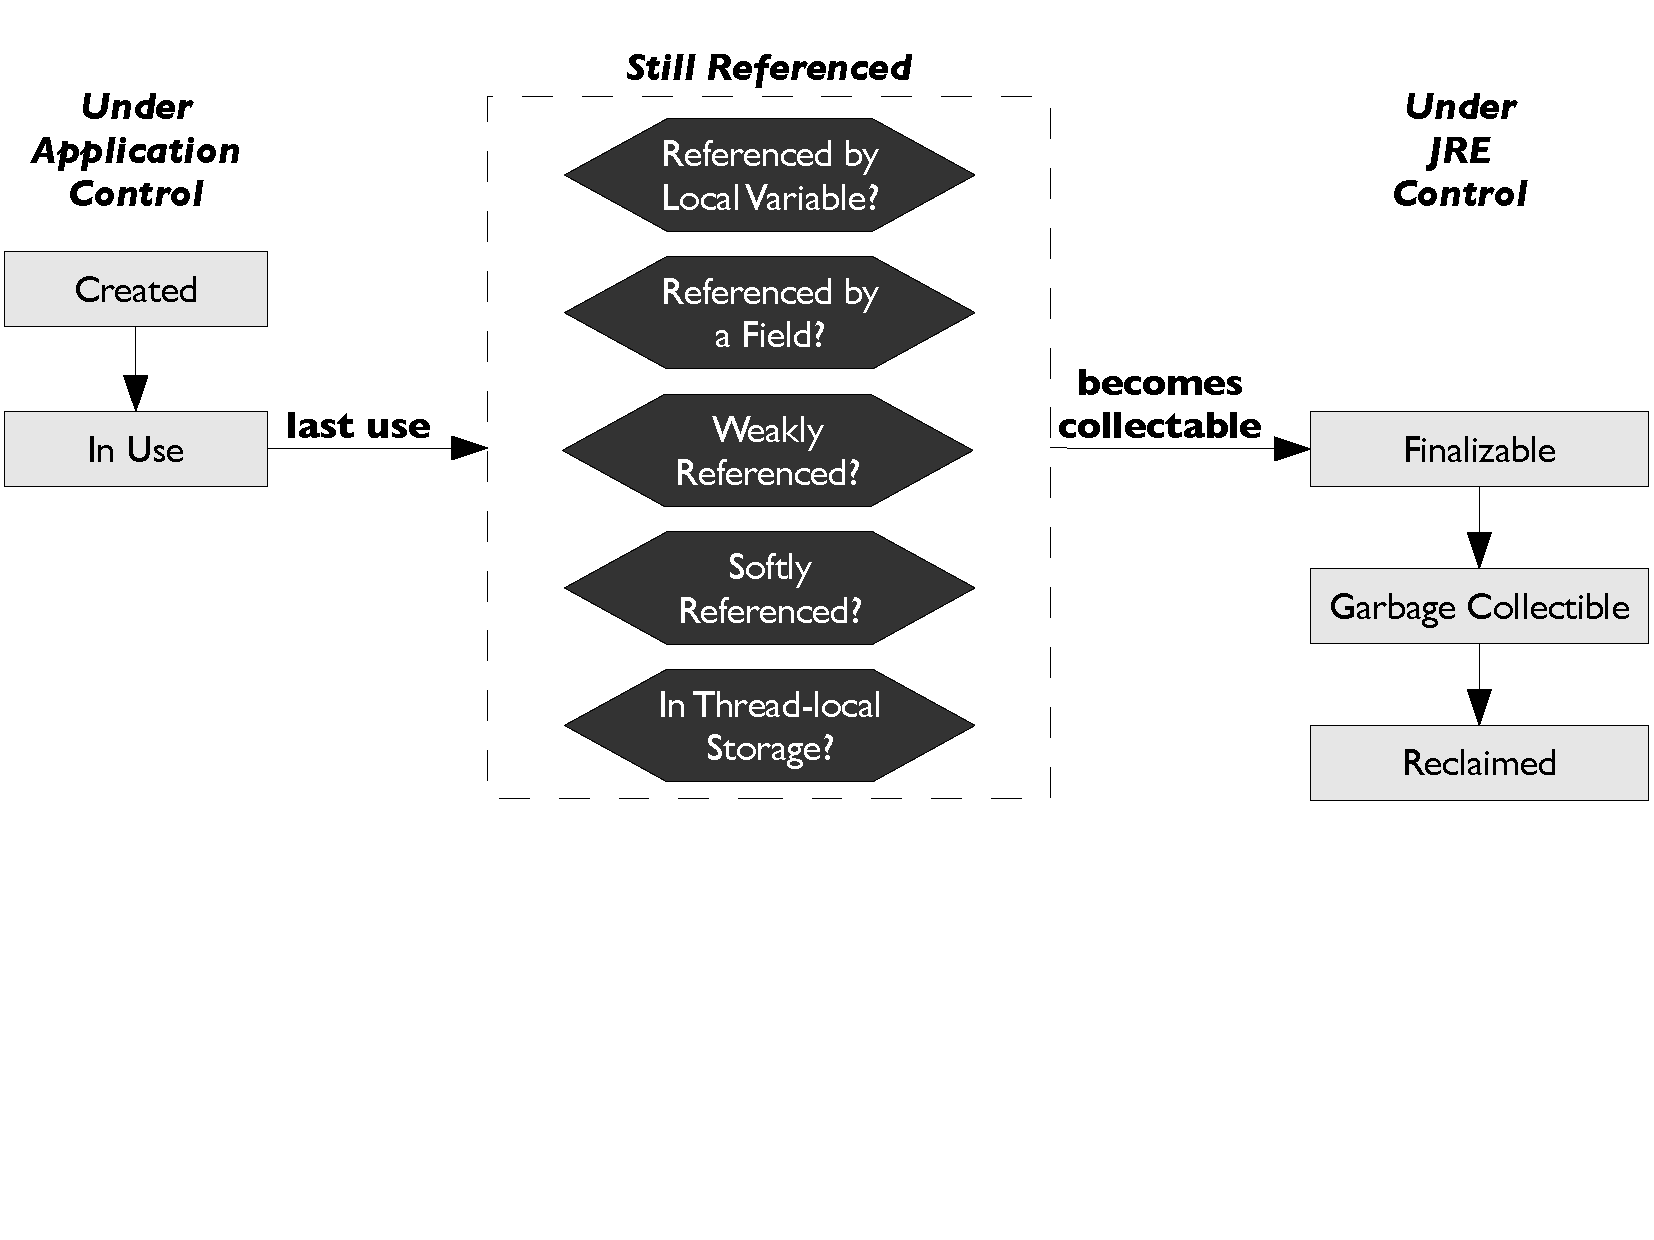
\includegraphics[width=\textwidth]{part4/Figures/lifetime/states}
	\caption{After its last use, an object enters a kind of limbo: the application
	is done with it, but the \jre hasn't yet inferred this to be the case. When an
	object exits limbo depends on the way it is referenced.}
		\label{fig:limbo-exit}
\end{figure}


\begin{comment}
\begin{figure}
	\centering
	\subfigure[The lifecycle of a typical object and its data.]{
	\label{fig:typical-lifecycle1}
			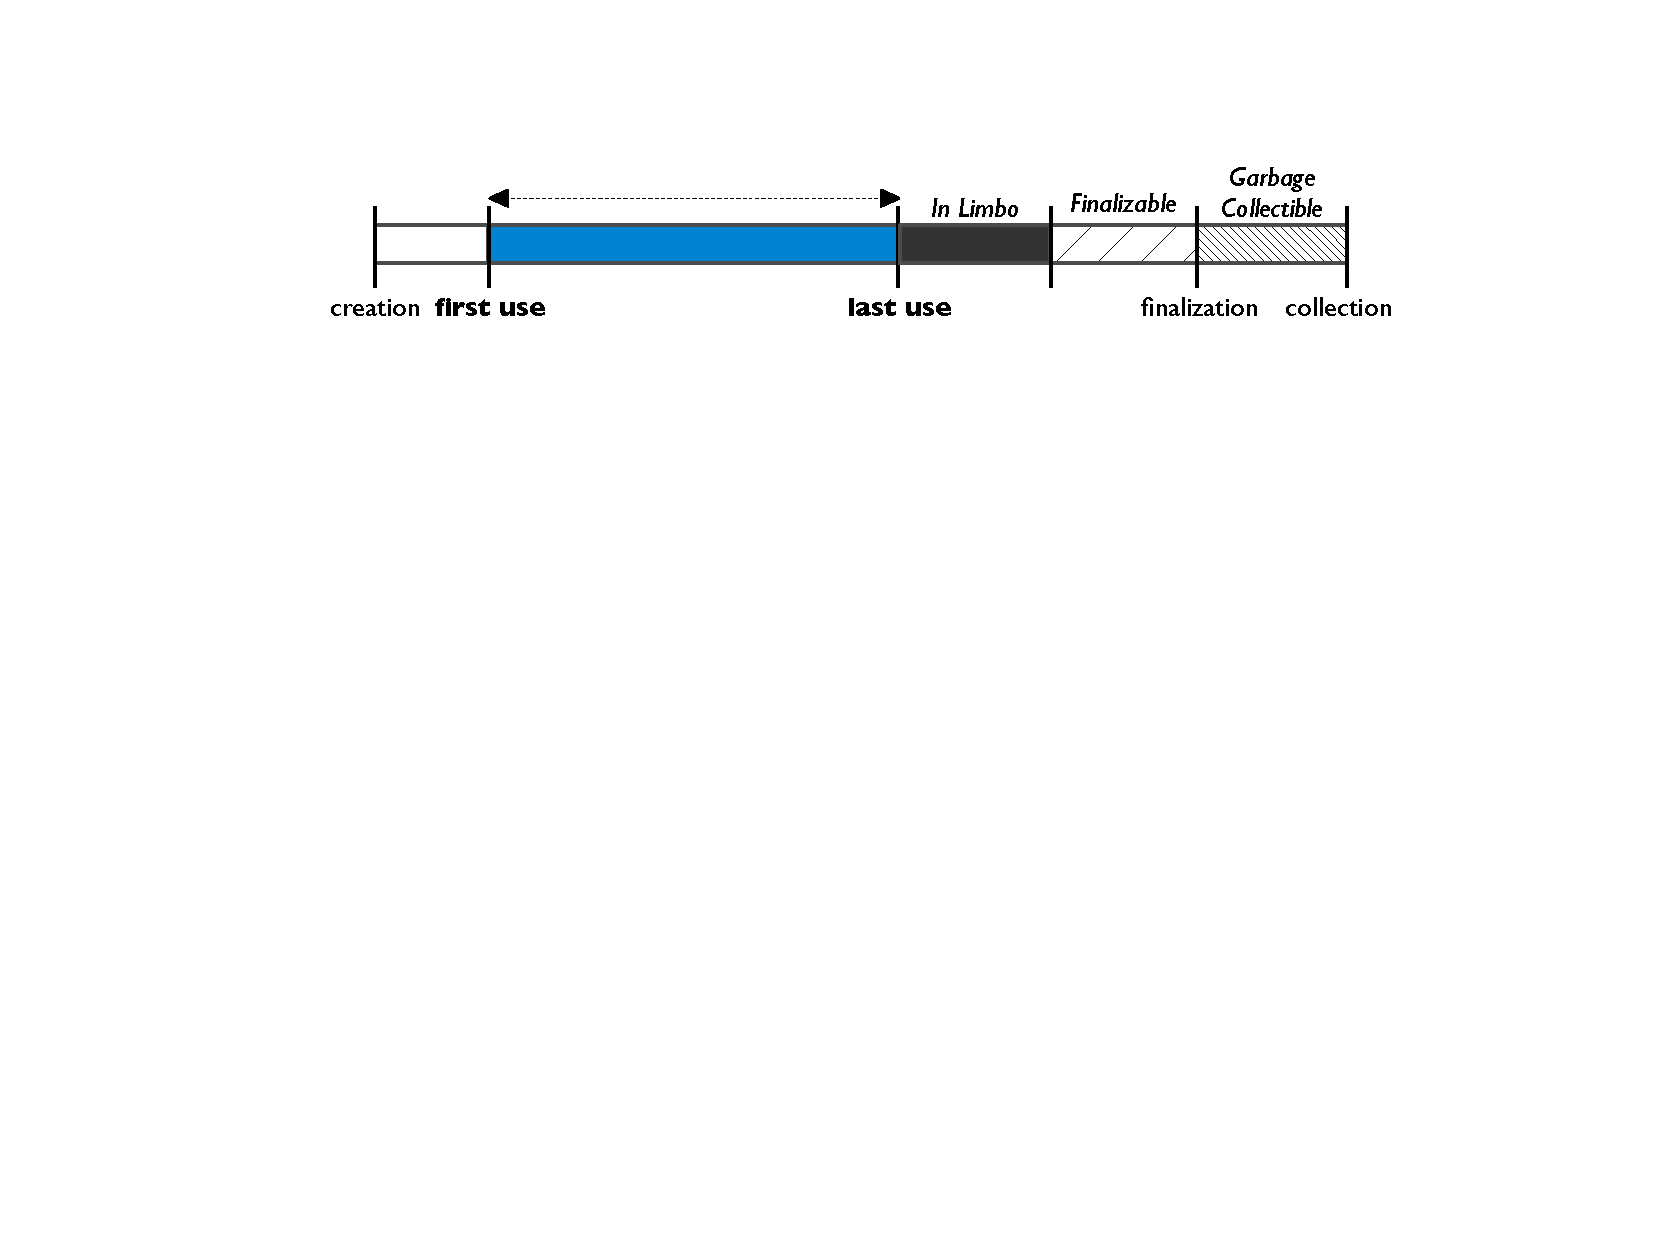
\includegraphics[width=0.95\textwidth]{part4/Figures/lifetime/object-lifecycle}
	}
	\subfigure[A situation where there are long periods between uses of an
	object's data.]{
	\label{fig:typical-lifecycle2}
		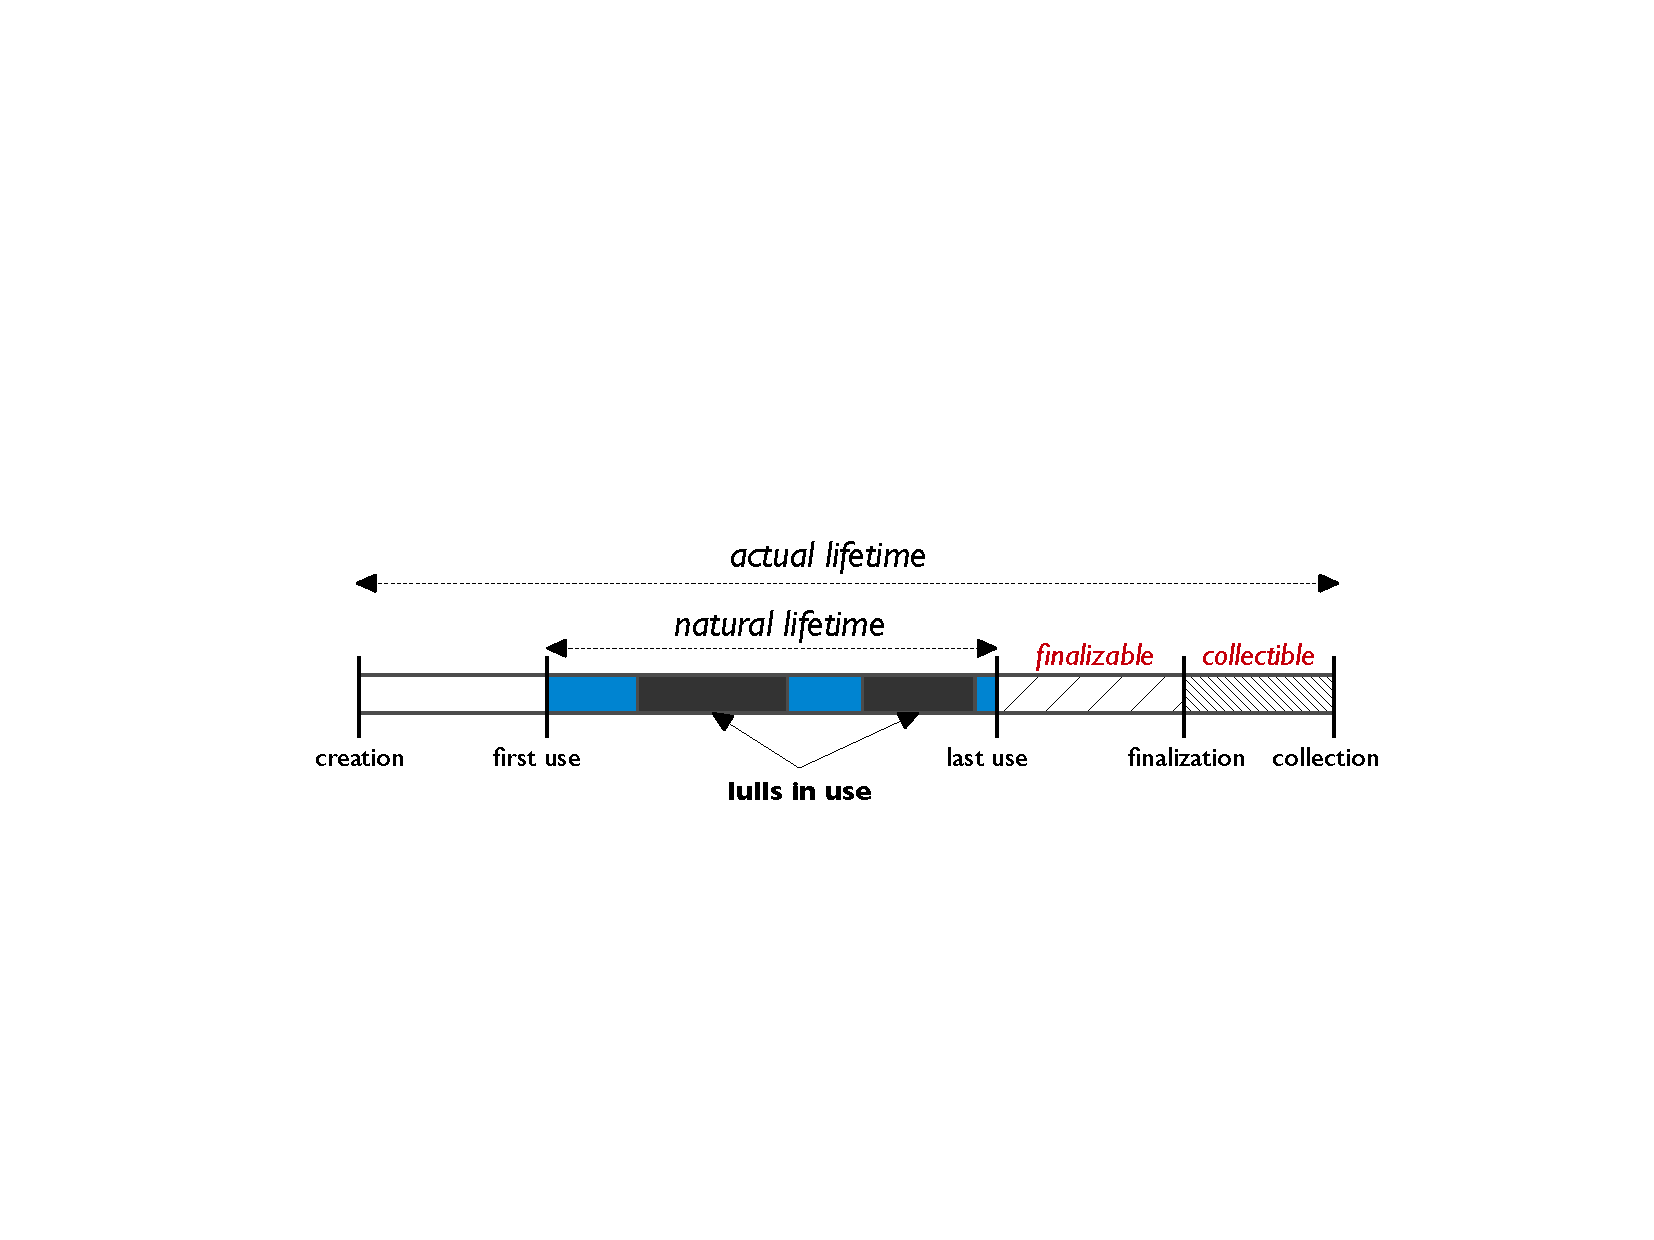
\includegraphics[width=0.95\textwidth]{part4/Figures/lifetime/object-lifecycle-lulls}
	}
	\subfigure[The lifecycle of the data  that is loaded from
	disk three times, and the objects that store it.]{
	\label{fig:typical-lifecycle3}
		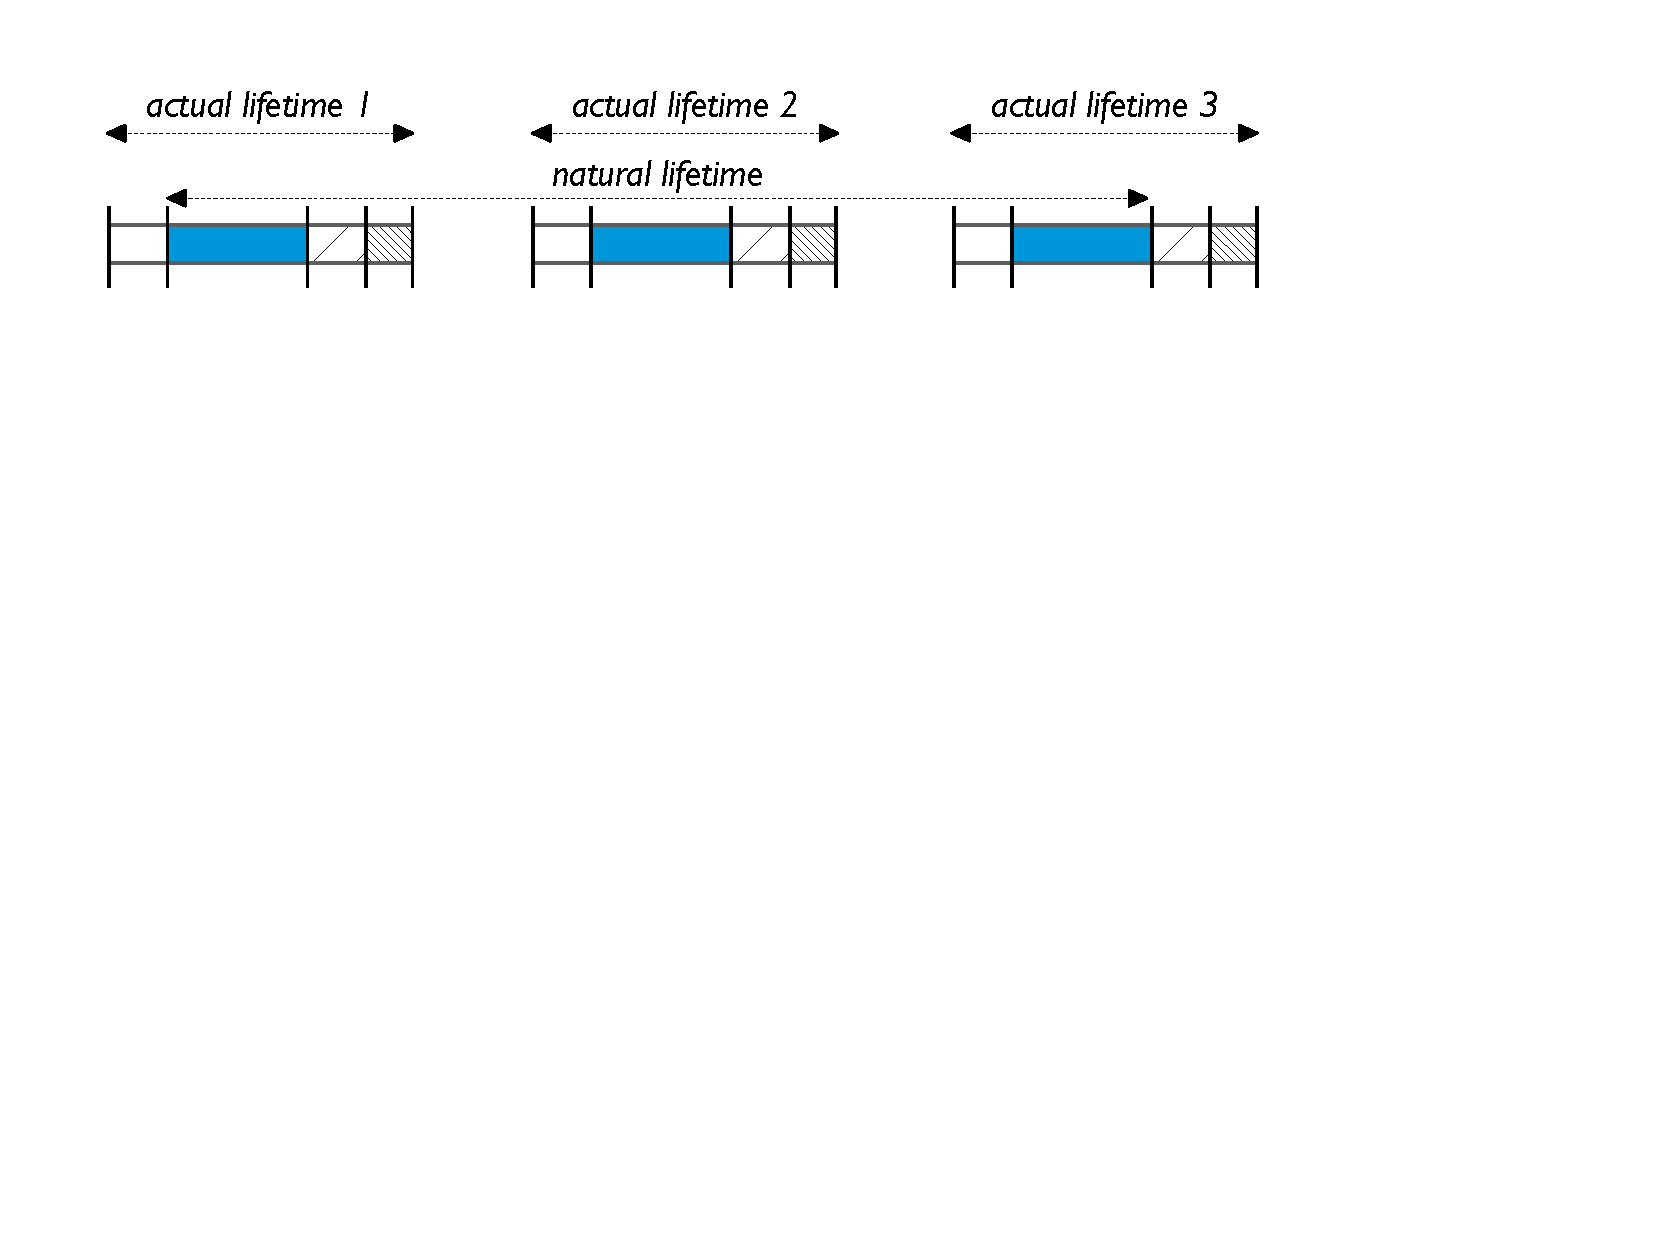
\includegraphics[width=0.9\textwidth]{part4/Figures/object-lifecycle2}
	}
	\caption{Examples of Natural and Actual lifetimes.}
	\label{fig:typical-lifecycle}
\end{figure}
\end{comment}


\section{Basic Management Mechanisms}
DO WE NEED THIS?

The point at which an object exits its limbo depends upon how it is referenced by
other objects. One can always assure that an object exits limbo by modifying your
code to overwrite all references to that variable. If an object is no longer
referenced at all, then it will exit limbo immediately.\footnote{Talk about
reference cycles?} For example, a common way to do this is by assigning
references to the value \code{null}. This is tricky in many cases, because it may not be easy to
know where all those references emanate from. Who is to say that, when one calls
the \code{parse} method of a \class{SimpleDateFormat} object, that it does not
squirrel away a reference to the \class{ParsePosition} passed as a parameter? The
API contract for \code{parse} makes no such claims, one way or the other. This is
certainly calls to mind the worst of the days of explicitly managing memory in a
language like C.


Still, one can't always rely on automatic mechanisms to guide an object out of
limbo in a timely fashion.
\autoref{fig:limbo-exit} and \autoref{tab:limbo-exit}
illustrate how an object may exit limbo. 
A garbage collector only knows that an object is ready to
be collected based on {\em reachability}: how the objects point to eachother.
If, as in the \class{ParsePosition}
or \class{SimpleDateFormat} objects from our example, the object is referenced
only by a local variable of a method, the \jre will not consider reclaming its
storage until the variable's scope exits; e.g. when the loop continues to the
next iteration, or when the method returns, depending on the scope of the
variable that references the object. If the object is referenced only by a
field of another object, then it must wait for that other object to exit limbo
before it can do so. 
An objects pointed to be only by a static field has a good chance of never
being collected. A class only exits limbo when it is unloaded by the \jres
class loading mechanism, which is unlikely to happen if it has static fields
that reference other objects. Therefore, unless that field is overwritten,
objects pointed to by static fields are likely never to exit limbo.
\section{Balancing Time and Space}
\label{balance-time-and-space}

sometimes we extend lifetime to optimize (for time)

sometimes we shorten lifetime to optimize (for space)



\begin{table}
\centering
\begin{tabular}{|l|l|} \hline
\em mechanism & \\ \hline \hline
resource pool & \\ \hline
cache & \\ \hline
sharing pool & (interning)\\ \hline
memoization & \\ \hline
backing store &(externalized memo) \\ \hline
non-OO & (column orientation) \\ \hline 
\end{tabular}
\caption{Lifetime management mechanisms not provided by the Java language that one must implement.}
\label{tab:software-lifetime-management}
\end{table}

\chapter{Correlated Lifetimes}

\begin{table}
\centering
	\begin{tabular}{ll} \toprule reachable only from  & moment
	when object exits limbo \\ \cmidrule(r){1-1} \cmidrule(l){2-2}
			%
			nothing & immediately
        	\\
        	%
        	local variable & after scope exits
        	\\ \addlinespace
        	%
        	instance field of an object & 
        	when that object exits limbo %(could be \emph{never} --- memory leak)
        	\\
        	%
        	static field of an object &
        	when that object's class is unloaded
        	%
        	\\ \addlinespace
        	field of \class{WeakReference} & immediately
        	\\
        	%
        	field of \class{SoftReference} & approximately
        	LRU%$^{**}$
        	%
        	\\
        	$\ldots$ with \class{ReferenceQueue} & $\ldots$ then, after removed
        	from queue
        	%
        	\\ \addlinespace
        	entry in thread local storage & when that thread dies
        	%
        	\\ 
        \bottomrule
    \end{tabular}
	\caption{When, or
	even whether, an object exits limbo depends upon how your program references
	it. If these references aren't explicitly overwritten, e.g. by your
	code expliclty assigning the reference to \code{null}, then an object only
	exits limbo under certain restricted circumstances.
%	The point when an object exits limbo depends on 
	%decisions under programmer control: it depends on how the object is
	%referenced.
	%older {\jre}s	use very poor heuristics for handling soft references; see the
	% body for more detail.
	%, it will be reclaimed
	%under certain rules, or may be part of a memory leak
	}
	\label{tab:limbo-exit}
\end{table}


There are important lifetime management policies that are not expressible via the
normal mechanisms. When referenced by a local variable, an object lives or dies
with the scope of the variable; when referenced by another object, it lives or
dies along with that object (both, of course, in the absence of overwriting a
reference). The Java specification provides three other mechanisms that let you
guide the \jre to the right time for an object to exit limbo: weak references,
soft references, and thread-local storage.

\section{Using Weak References}
\index{Weak Reference}

Java provides a low-level mechanism that one can use to implement a
correlated lifetime memory management policy, in the form of weak references.
The standard library exposes this feature in the class
\class{java.util.WeakReference}. Using this class correctly is
difficult, because the semantics of weak references does not directly map to
any important application-level use cases.

\begin{definition}
When calling the constructor \class{new WeakReference(obj)},
 this new instance will maintain a reference to \code{obj}, however
 \code{obj} will exit limbo, and become a candidate for cleanup processing by 
the \jre, as if that reference did not exist.
\end{definition} 

When used in this way, weak references don't keep an object alive longer than it
otherwise would have, in the absence of weak references. 
This seems pretty far from anything an application might
need. Still, you can use this low-level feature to implemented correlated
lifetime, as long as you're careful. 
When used to implement correlated lifetime policies, weak references may
indeed delay the time till an object exits limbo.
Improper use of a \class{WeakReference} will
render your code worse off than before. It is quite possible that you will not
have achieved the correlated lifetime that you need, but in a way that is hard
to tell. Even worse, when using weak references, you can introduce memory
leaks. Be very cautious when using them, and follow these rules.

\callout{weaks}{Rules for Using \class{java.util.WeakReference}}{
	In order to assure that you use of weak references works properly, you must
	follow three rules:
	\begin{itemize}
      \item Your instances of \class{WeakReference} must not, directly or
      indirectly, maintain a non-weak reference to the object you wish to
      annotate. It is best to maintain a collection of non-weak references to
      the annotated objects, and use a local variable, or a subclass of
      \class{WeakReference} for any other ways you refer to the annotated object.
      
      \item You must ensure that the \class{WeakReference} objects (or
      subclasses thereof) that you create will exit limbo no sooner than the
      annotated objects. Otherwise, these objects themselves, following the
      rules of \autoref{tab:limbo-exit}, will exit limbo too early. So, if the
      annotated objects are referenced by a collection that is in turn
      referenced by a static field, then the same must be true for the weak
      reference objects as well. 

      \item Since you have to maintain two, parallel, collections to maintain
      references to the annotated objects, and to the annotations, you must
      ensure that exit limbo in lockstep. It is best to create your instances
      of \class{WeakReference} with a \class{ReferenceQueue} parameter. You
      must periodically call \code{poll} on this queue, and remove the
      \class{WeakReference} instances from the parallel registry.
    \end{itemize}
}

You can see that, despite the benefit of some support from the \jre, there
is quite a bit of memory management that you are left with. Luckly, the
standard library ships with a \class{WeakHashMap}\index{WeakHashMap} which deals
with some, but not all, of the legwork of managing weak references. It will
handle the second and third items, but not the first. It is still up to you to
ensure that none of your annotations, directly or indirectly, reference the
annotated object. 

\begin{example}{Timestamp Annotation}
How can you associate a timestamp with an object in a way that avoids memory
leaks and that scales well to a highly concurrent workload?
\end{example}

We can start with the following code:

\begin{shortlisting}
class TimestampAnnotation<T> {
	T t;
	long timestamp;
}
List annotations;
for (String string : inputList) {
	...
	annotations.add(new WeakReference(new Wrapper<String>(string)));
	...
}
\end{shortlisting}

Despite your use of \class{WeakReference}, you would find that neither the main
object (the strings), nor the annotations, would ever be collected. This code
has two memory leaks. One of the leaks is due to a
violation of the first principal of the use of weak references: the annotations
strongly reference the objects being annotated. It is not always this easy to
debug problems in using weak references. Your application will hold on to objects
that you didn't expect. Quite often, it is difficult to even know that there is a
problem in the first place! The application may behave normally, except that it
will consume more memory than necessary; if this extra memory consumption pushes
it over your maximum heap size, then your application will crash --- you will
know something is wrong, but diagnosing this type of problem, a memory
leak\index{Memory Leak}, is quite difficult. It is better to keep the
three principles of weak references in mind, and design in a way that avoids
memory leaks in the first place. Your annotations can be modified to use a
\class{WeakReference} to the main object:

\begin{shortlisting}
class TimestampAnnotation<T> {
	WeakReference<T> t; // annotation only weakly refs main object
	long timestamp;
	
	TimestampAnnotation(T t) {
		this.t = new WeakReference(t);
	}
}
\end{shortlisting}

In this case, the annotation has no normal references to the annotated object,
and so it obides by the first rule of weak references. If you remember from
\autoref{chapter:delegation}, the code can be improved further to avoid the cost
of delegation. This version of the annotation class extends
\class{WeakReference}:

\begin{shortlisting}
class TimestampAnnotation<T> extends WeakReference<T> {
	long timestamp;
	
	TimestampAnnotation(T t) {
		super(t);
	}
}
\end{shortlisting}

Unfortunately, both of these updated versions h



\section{Using Finalizers}


\section{Correlation Gone Wrong: Memory Leaks}
\index{Memory Leaks}
%about objects not information; we can discuss in outside the box the issue of
%information needed forver but shuttled in and out.

\chapter{Extreme Scalability of Long-lived Data}
\label{chapter:large-long-lived}

All of the tuning advice presented so far in this book can only get you so far.
Sometimes, despite your best efforst of tuning entities and collections, your
application's objects still do not fit into the memory constraints of the target
platform. Managing a great number of long-lived objects therefore comes with its
own set of challenges, even though objects these objects are free from the bugs
that riddle those with correlated lifetime. To manage objects that, after a
reasonable amount of tuning, still don't fit into the heap, you have three
solutions at your disposal: throw hardware at the problem, implement a kind of
demand paging, or code your data models in a non-object oriented way.

\paragraph{Buy More Memory} The first solution you may consider is buying more
memory for the target platform. If your budget allows for this, then by all means
you should strongly consider doing so. There are some downsides to keep in mind.
The first is heap size limits. At some point, you will need to switch from a
32-bit JVM to a 64-bit JVM\index{64-bit}. This switch will result in a large
increase in overhead. As discussed earlier, the amount of blowup resulting from a
switch to a 64-bit JVM depends on the degree of delegation in your data models. A
64-bit JVM only adds overhead to the extent that your data models have headers
and pointers. The alternative, running with compressed
references\index{Compressed References}, limits you to around 32GB of memory, and
imposes a few percent slowdown. In addition, running with a large heap can result
in increases in the length and fluctuations in pause times.

\paragraph{Shuttle Objects in and Out of the Java Heap} Rather than attempting to
fit all of your objects into a single heap, you can store them outside of the
Java heap, and swap them in (and out), on demand. If the logic of your
application allows for recomputing the data stored in these objects, you need to
be careful to compare the recreation cost with the costs of marshalling objects.
You can choose to marshall objects to and from a local disk, or you can use one
of several frameworks that provide a distributed key-value map.

\paragraph{Break the Java Mold} Despite being an object-oriented language, there
is nothing in the Java language that prevents you from storing objects in a
non-object oriented way --- nothing, that is, except programming time and
maintenance expense. It is possible to store data only in arrays, as one would in
a language such as Fortran, and retain a great deal of object orientation in your
data models and programming interfaces. 

This chapter presents a methodology for predicting the scalability of your data
models, and presents several solutions to demand-marshalling objects, and for
storing objects in a ``Fortran style''.

\section{Scalability: Quantitative Methodology}

\begin{figure}
\centering
	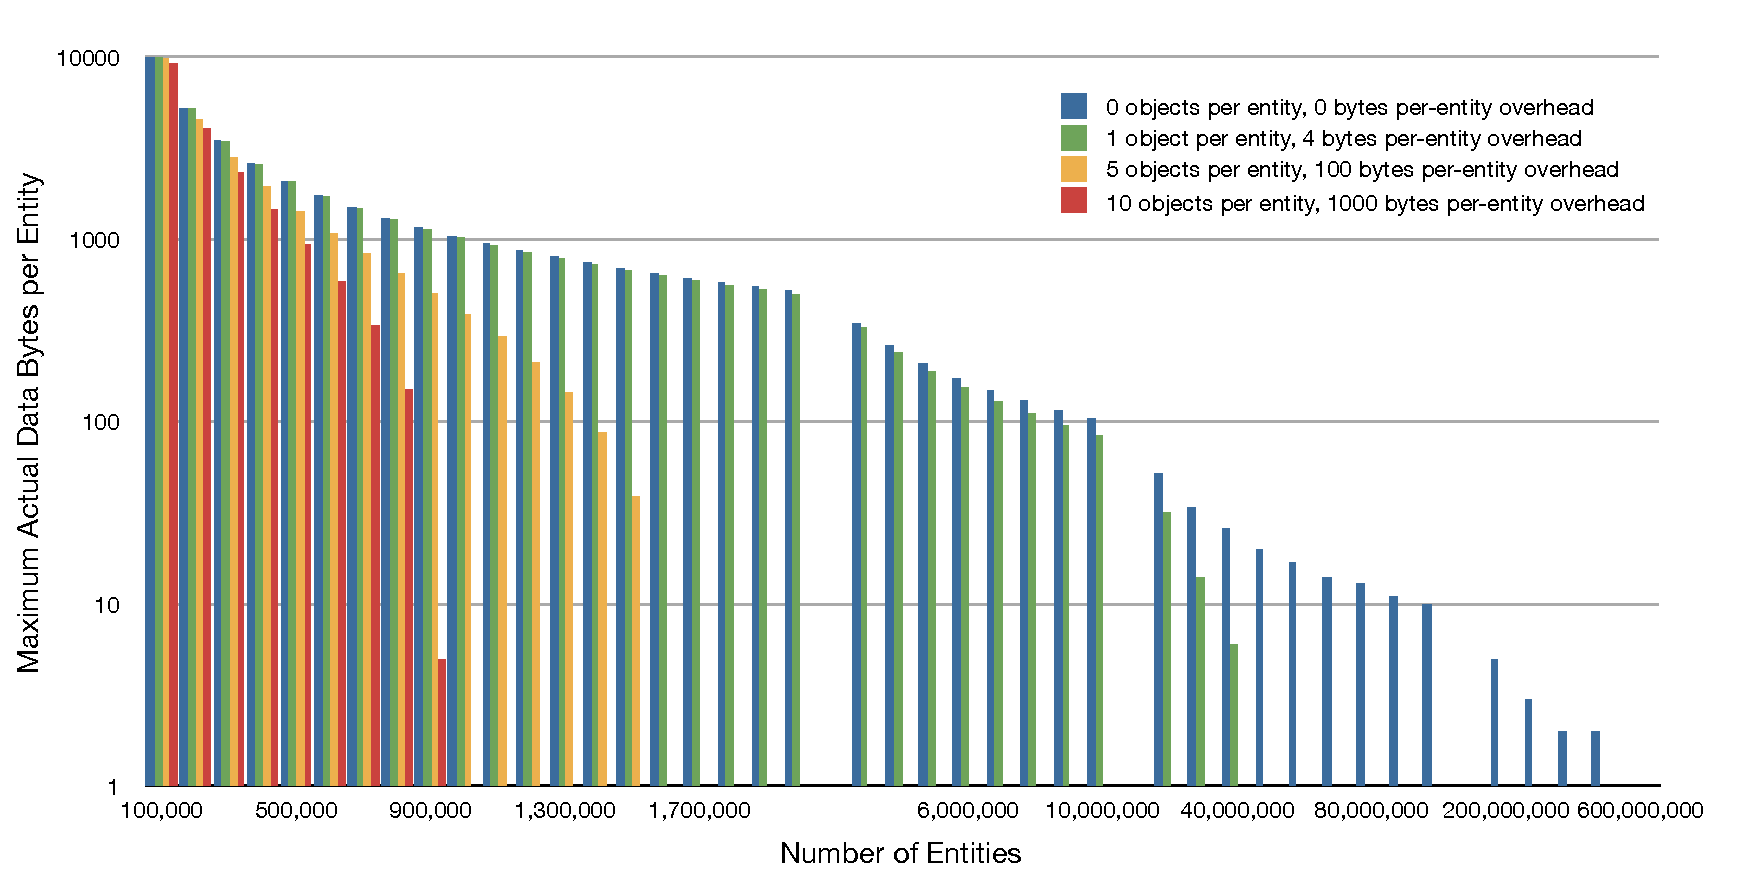
\includegraphics[width=\textwidth]{part4/Figures/maxActualData}
	\caption{The amount of actual data you can store in your entities depends on
	the degree of delegation in your entities, and the per-entry overhead of the collection in which these entities
	reside. This chart assumes a limit of 1 gigabyte of Java heap.}
	\label{fig:maxActualData}
\end{figure}

TODO: write this section, explaining \autoref{fig:maxActualData}, or delete it.

\section{Bulk Sharing of Immutable Data}
\label{sec:bulk-sharing-pool}
\index{Bulk Sharing Pool}

Primitive arrays are often the repository for most of your application's actual
data. If your application has a few large primitive arrays, then the overhead of
the arrays will be dwarfed by the actual data contained therein. A common problem
with Java applications is that they have many small primitive arrays.
\index{Small Primitive Arrays} If the large majority of your actual data is in
these primitive arrays, and the average length of each array is 10 characters,
then your application will have a memory bloat factor of 61\%
% 16/(10 + 16)
--- almost half of your heap will be wasted on the object headers of the
primitive arrays. The problem grows worse if these primitive arrays are wrapped
inside of objects such as \class{String} or \class{ByteArrayOutputStream}. If
wrapped inside of \class{String} objects, then your application is doomed to a
memory bloat factor of 83\%.
% (16+32)/(10+16+32)

If these primitive arrays store only a small number of distinct sequences, this
problem of high overhead can, at least indirectly, be addressed by
interning.\index{Interning} Earlier, \autoref{sec:sharing-strings} discussed
string interning. If your primitive data is string data, then you can use the
\jres built-in mechansm for pooling this data, so that only one copy of each
string is kept in memory. For non-string data, you will have to roll your own
solution. In any case, however, interning only tackles a part of the problem at
hand. By keeping only a single canonical copy of the primitive data, you
eliminate the primitive array headers for the duplicates.
\autoref{fig:bulk-sharing-pool}a and \autoref{fig:bulk-sharing-pool}b illustrate
a simple case of interning. Of three strings, there are two duplicate ``grape''
sequences. The residual high overhead is due to the remaining primitive array
object headers, and all of the \class{String} objects; none of the \class{String}
objects are eliminated by interning. Interning removes only the duplicate
primitive array overheads.


\begin{figure}
\centering
	\subfigure[Three normal	\class{Strings}.]{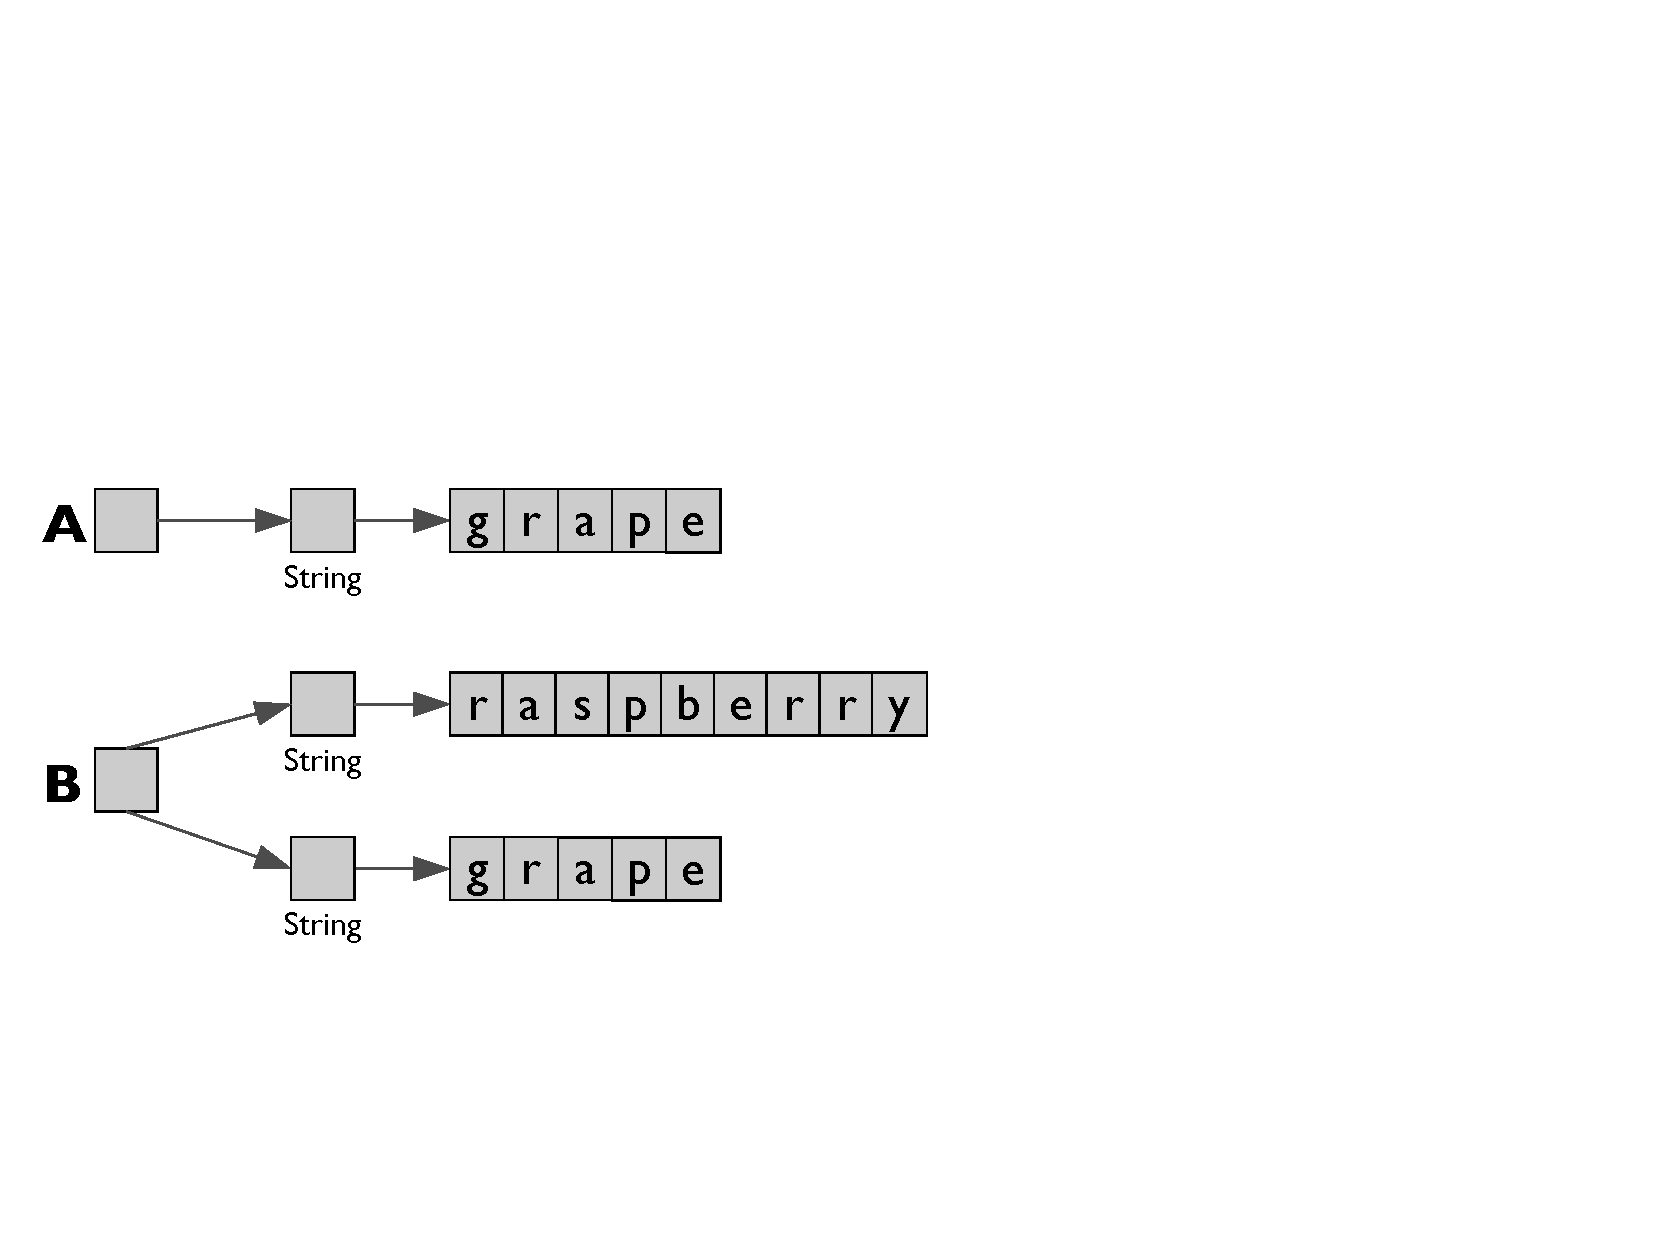
\includegraphics[width=0.425\textwidth]{part4/Figures/bulksharingpool1}}
	\qquad
	\subfigure[Interning.]{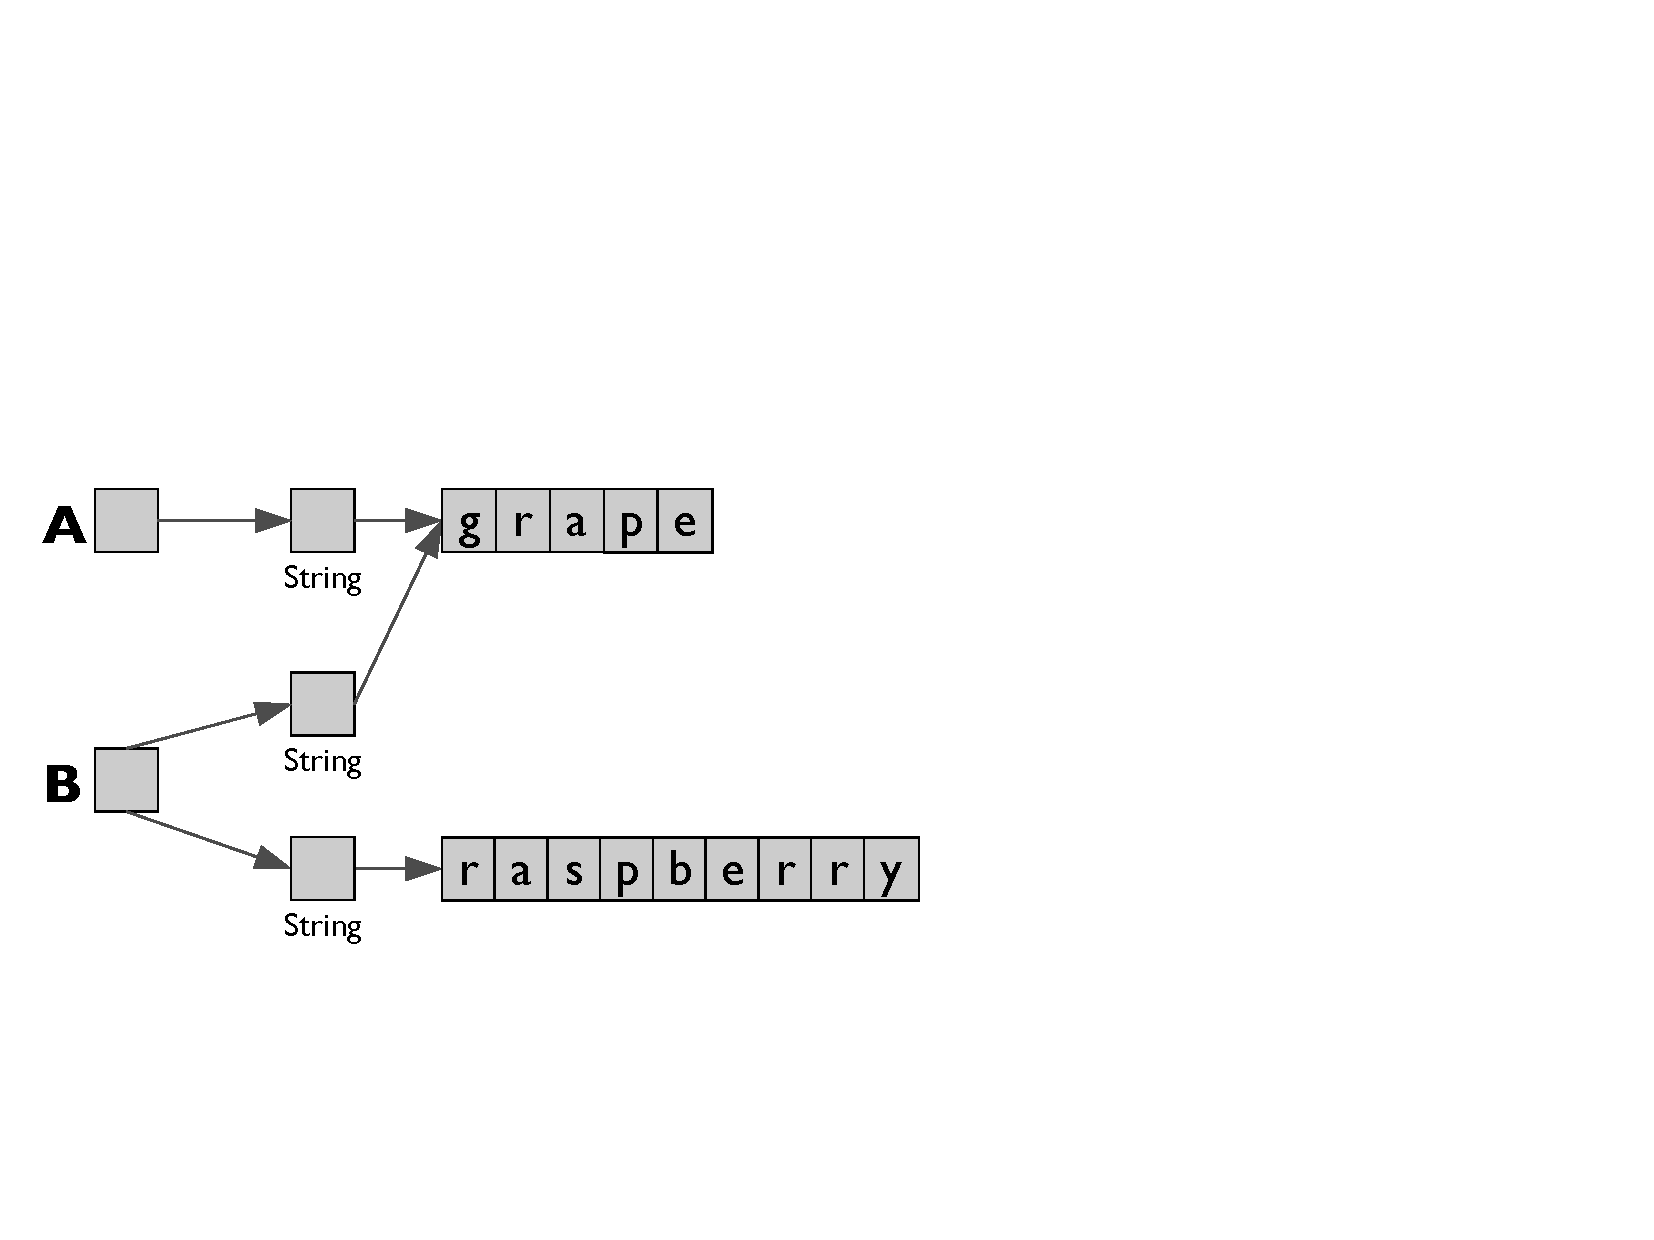
\includegraphics[width=0.425\textwidth]{part4/Figures/bulksharingpool2}}
	\qquad
	\subfigure[Bulk	sharing	pool.]{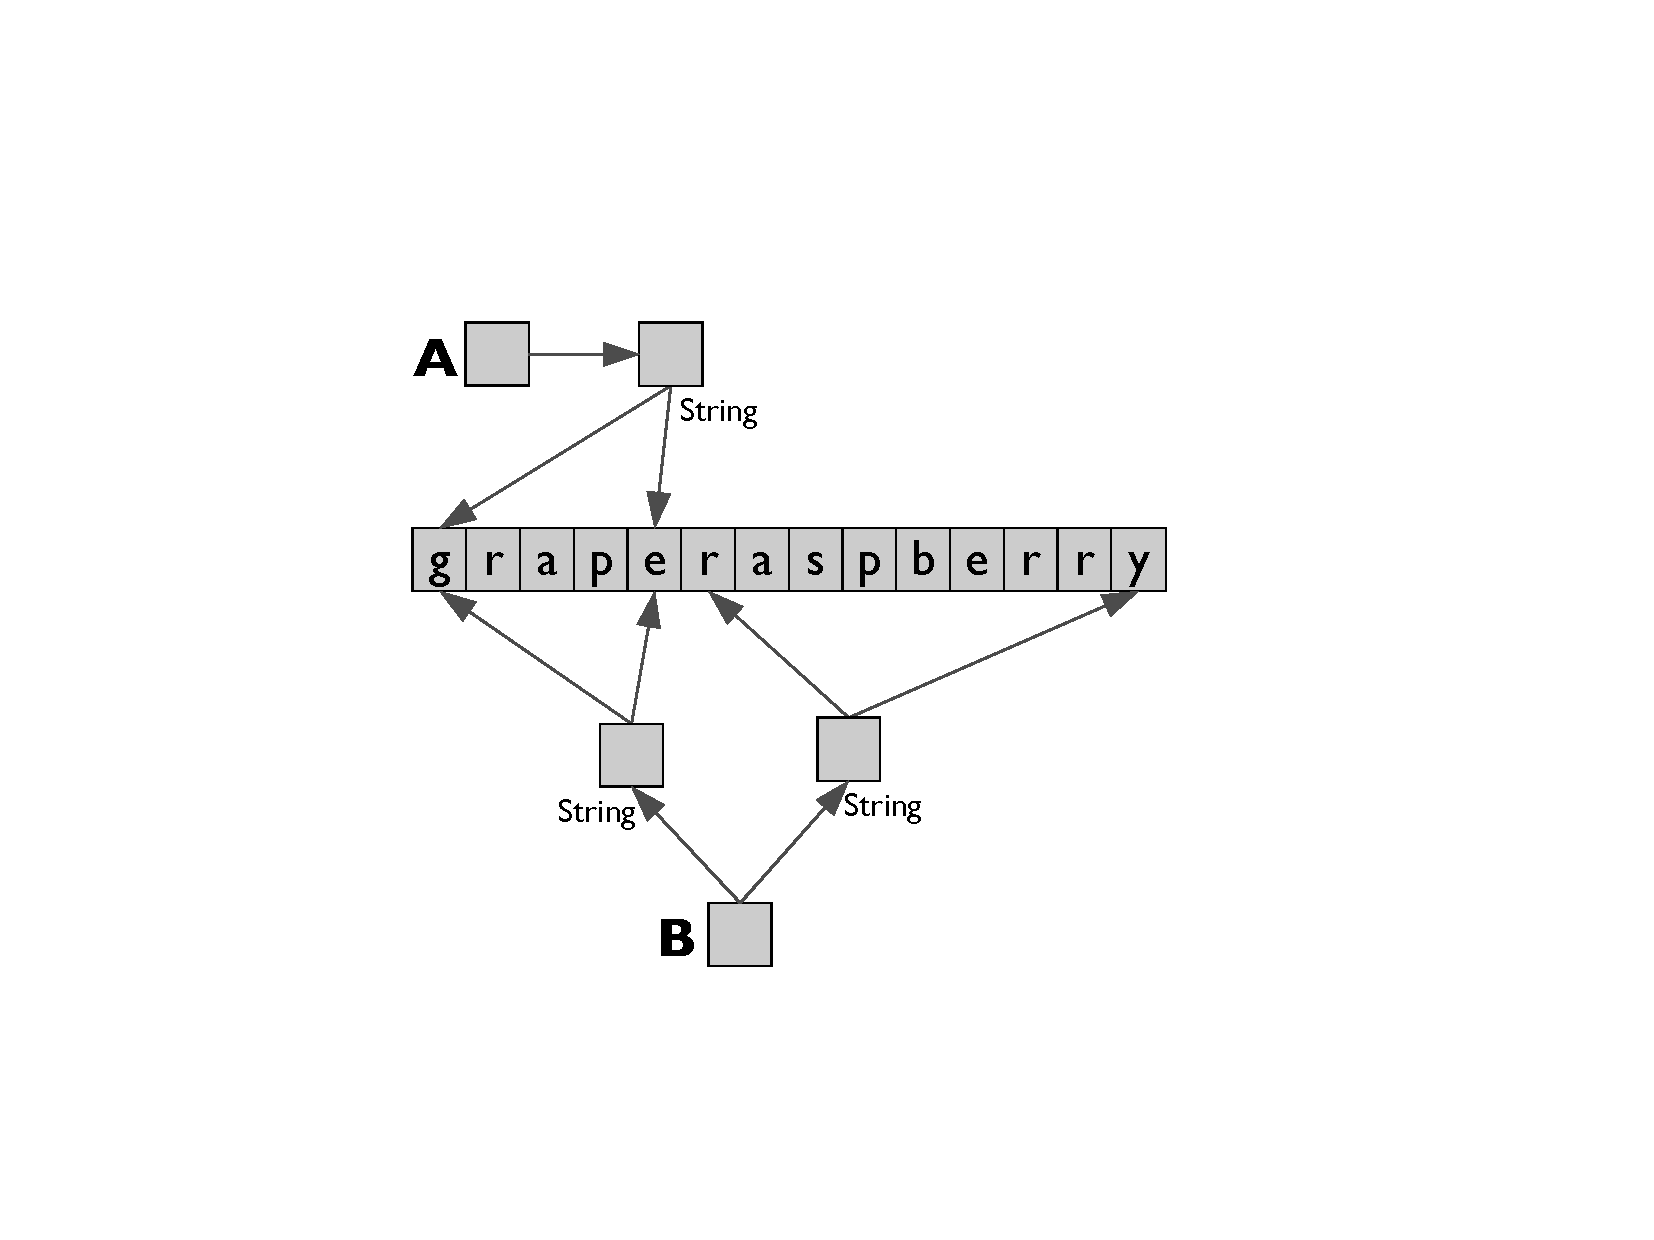
\includegraphics[width=0.36\textwidth]{part4/Figures/bulksharingpool3}}
	\qquad
	\subfigure[Bulk	sharing	pool, no wrappers.]{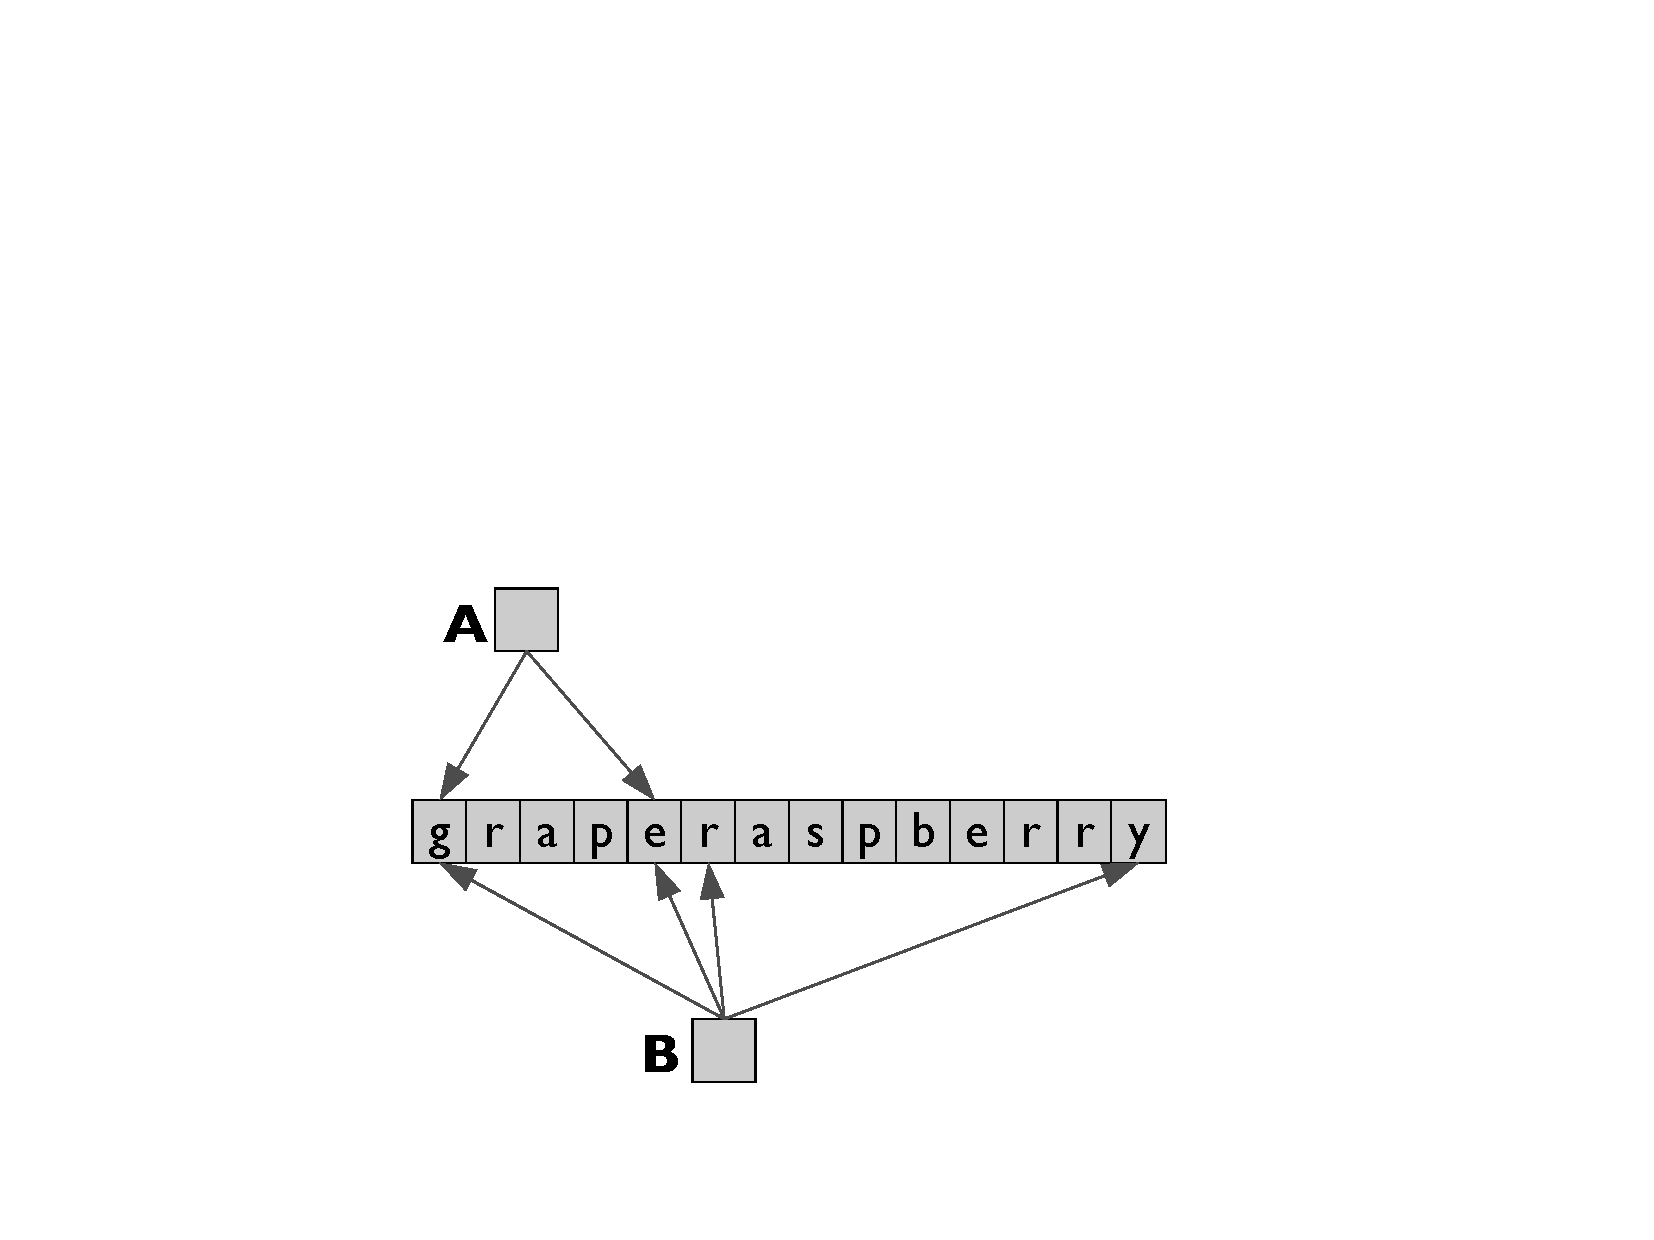
\includegraphics[width=0.36\textwidth]{part4/Figures/bulksharingpool4}}
	\subfigure[The memory consumed by one million strings, each of length 10
	bytes, for varying degrees degrees of distinctness; e.g. 10\% means that
	there are only 100,000 distinct strings.]{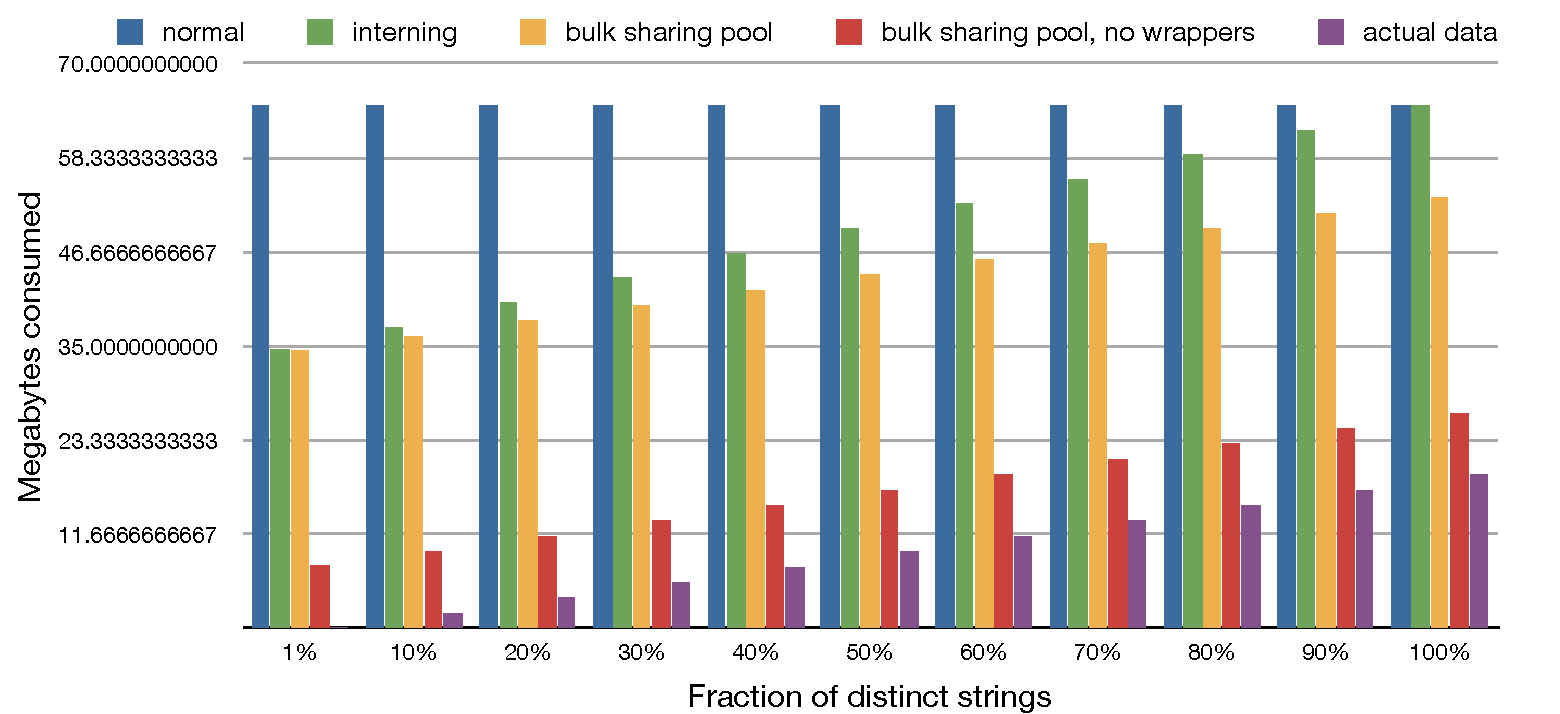
\includegraphics[width=\textwidth]{part4/Figures/bulksharingpool_consumptionchart.pdf}}
	\caption{If your application has many long-lived, but small, arrays of
	primitive data, it could suffer from high overhead. Interning avoids
	duplication. On top of interning, a Bulk Sharing Pool offers the additional
	potential for you to eliminate the primitive array wrappers, and so can be
	beneficial if there are still a large number of unique sequences.}
	\label{fig:bulk-sharing-pool}
\end{figure}

By eliminating many duplicates via interning, you stand to save a large amount of
memory, but your memory bloat factor will still be quite high. Instead of a bloat
factor of 83\%, with interning your heap will have a bloat factor of at least
88\%.
% 3*(16+32)/(10*2+3*(16+32))
This value is a lower bound, because there is another curious problem that arises
when handling duplicate data. If there is a bounded number of distinct sequences,
but an increasingly large number of total sequences, your memory bloat factor can
approach 100\%. In this case, the per-sequence memory overhead grows with the
number of sequences, but the amount of actual data is bounded by the number of
distinct sequences.

There are two further optimizations open to you, but these require deeper
changes. Both optimizations store all of the sequences in a single, large array.
This storage style is an example of optimizing for a bulk of uniformly typed data
that is accessed in a uniform, and stylized, fashion. Why pay the expense of many
small primitive arrays, if your code does not need each sequence to be a Java
object? If you will never synchronize or reflect on sequences, as objects, then
the primitive array header is a needless expense.
\autoref{fig:bulk-sharing-pool}c illustrates this bulk storage of the sequences
in a single large array. You pay the primitive array overhead just once, across
all pooled sequences, rather than for every sequence. 
%In this case, your heap
%will have a memory bloat factor of
% 3*(16+32)/(10*2+3*(16+32))

To achieve the ultimate in memory efficiency, you must also eliminate the
\class{String} wrapper objects. This last step requires the most work on your
part. If you have the luxury of modifying the class definitions for the objects
that contain the string wrappers, then you can replace every pointer to a string
with two numbers. These numbers store indices into the single large
array of bulk data, and demark the sequence that the string wrapper would have
contained. You are essentially inlining the offset and length fields that every
Java \class{String} object has, and doing away with the hashcode field and the
extra header and pointers. This eliminates almost all sources of overhead.

\autoref{fig:bulk-sharing-pool}d charts the memory consumption of the four
implementations: using normal Java \class{Strings} without any attempt to remove
duplicates; using Java's built-in string interning mechiansm; using a bulk
sharing pool; and using a bulk sharing pool without any \class{String} wrappers.
The chart also includes a series comparison with the amount of memory consumed by
actual data.  The chart shows memory consumption of each implementation for
varying degrees of distinctness of the strings, for an case with one million
strings of length 10 characters each.
For example, if 500 thousand of the million strings are distinct (which
corresponds to the 50\% point in the chart), the normal implementation consumes
65 megabytes, the interning implementation consumes 50 megabytes, the bulk
sharing pool implementation consumes 44 megabytes, and the bulk implementation
without string wrappers consumes 17 megabytes. There are 500 thousand
distinct characters, so the actual data consumes about 10 megabytes.

The chart makes it pretty clear how much a few headers and pointers can affect
the scalability of your application. With only a bit of work, you can have an
implementation that scales very well, with only minimal overhead on top of the
actual data.

\section{Representing Relationships}

When representing relationships between entities, using standard object oriented
practices, you are severely limited in the number of entities and relationships
that you can store. Doing so in a straightforward manner, one that obeys object
oriented practices, is very similar to the task of representing a graph of nodes
and edges. For example, when caching data from a relational database in the Java
heap, the entities (rows in a database table) and relations (columns that contain
indices into tables) become the nodes and edges in a graph.

%\begin{example}{Storing a Graph}
If a graph has a great many nodes and edges, you must design its storage
carefully. Consider the small example illustrated in 
\autoref{fig:exampleGraph}. There are several ways to implement the abstract
data types, of nodes and edges, shown in that figure. Each strategy has its
positives and negatives, depending on whether ease of maintenance or memory
consumption are of primary importance.
%\end{example}

\begin{figure}
\centering
\subfigure[Example graph.]{
\label{fig:example-storing-relations-graph}
\shortstack{
	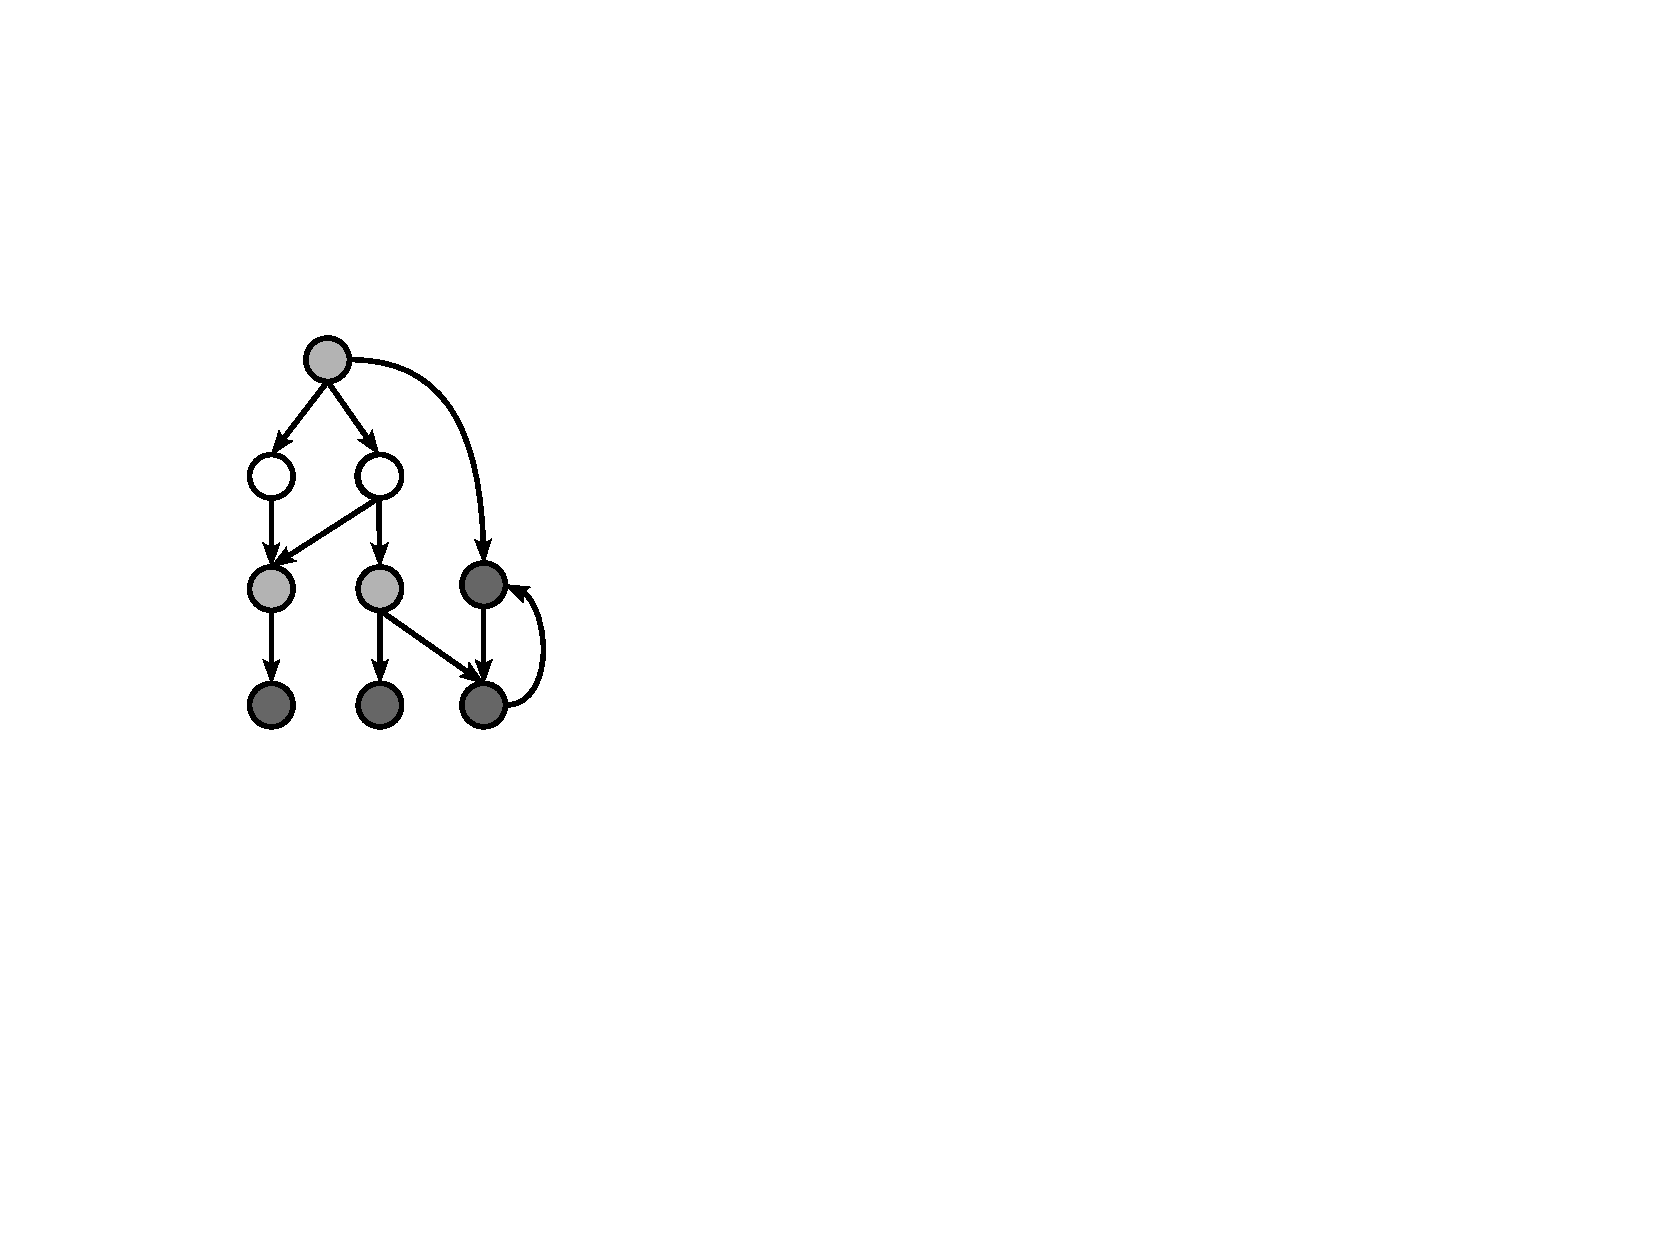
\includegraphics[width=0.3\textwidth]{part4/Figures/exampleGraph}
	\\ \vspace{5mm}
	}
}
\qquad
\begin{subfloat}
\label{fig:graph-interfaces}
\begin{minipage}[b]{0.45\textwidth}
\begin{figurelisting}
interface Graph {
	Set<Node> getNodes();
	Set<Edge> getEdges();
}
interface Node {
	Color getColor();
	Set<Edge> getChildren();
	Set<Edge> getParents();
}
interface Edge {
	Node getFrom();
	Node getTo();
}
enum Color {
	White, LightGray, DarkGray
}
\end{figurelisting}
\end{minipage}
\caption{Abstract data types for nodes and edges.}
\end{subfloat}
	\caption{An example generic graph of three colors of nodes.}
	\label{fig:exampleGraph}
\end{figure}

\begin{figure}
\centering
\begin{subfloat}
\begin{minipage}[b]{0.3\textwidth}
\begin{figurelisting}
class Node {
   Color color;
   Set<Edge> parent;
   Set<Edge> child1;
   Set<Edge> child2;
}
\end{figurelisting}
\end{minipage}
\caption{Concrete classes}
\end{subfloat}
\quad
\begin{subfloat}
\begin{minipage}[b]{0.5\textwidth}
\begin{figurelisting}
public Node(Color color) {
   color = color;
   parents = new HashSet<Edge>();
   children = new HashSet<Edge>();
}
\end{figurelisting}
\end{minipage}
\caption{Node constructor that uses the default \class{HashSet} constructor.}
\label{fig:node-obvious-constructor}
\end{subfloat}
\caption{A straightforward implementation of the Node interface.}
\label{fig:node-obvious-impl}
\end{figure}

\autoref{fig:graph-interfaces} shows the interfaces for a \class{Graph},
\class{Node}, and \class{Edge} that one must implement. A common implementation
strategy, applied to the \class{Node} and \class{Edge} data types, is a
straightforward mapping of interfaces to concrete classes.
\autoref{fig:node-obvious-impl} shows such an implementation for the
\class{Node} data type. Following this
strategy, the \class{Node} class has three fields, to store its \class{Color}
and the relations to children and parents; these relations are implemented with a
standard collection, likely a \class{HashSet}. The \class{Edge} class has two
fields, to store pointers to the source and target nodes. This implementation is
easy to implement. It is also easy to maintain: changes to the interfaces can be
directly mapped to changes to the implementation, because the two are parallel
versions of each other. The nodes and edges, and relations between them, are
objects that can be manipulated using normal object oriented practices; e.g. you
can write \texttt{node.getChildren().get(5).getTo()\-.getColor()}, which reads
as a fairly natural, albeit verbose, expression of what you intend.

\paragraph{A Straightforward Implementation}
Without any thought for memory concerns, the constructor for a node would be as
shown in \autoref{fig:node-obvious-constructor}. In this implementation, the
memory cost per node is three pointers plus two collections of default size. As
\autoref{tab:collection-costs} shows, the the default constructor of a
\class{HashSet} allocates an array to hold 16 elements; the per-collection cost
is 136 bytes and the per-entry cost is 28 bytes. If, on average, a node has one
parent and 2 children, then each node will consume one object header plus $3*4
+2*136 + 2*3*28$, or $464$ bytes; using \class{ArrayList} instead of a hash map
would cost $3*4+ 2*(80 + 10*4)$, or $264$ bytes. Both choices result in 24\% of
memory wasted on null pointers.
% hashset: 112=14 entries at 4 bytes each, times two for parents and children 
% arraylist: 68=8 entries at 4 bytes each, times two for parents and children
The 136 bytes (29\%) spent on the parent collection is unnecessary, for those
nodes that have exactly one parent. Even an optimally structured set which
includes just one pointer for a set with one entry would still impose two pointer
costs to reference a single parent node: one pointer to reference the set, one
for the set to reference the parent node.

In addition to the cost of the nodes are the cost of the edges objects. By
objectifying each edge, this implementation pays a cost of one object header
plus two pointers, or 24 bytes (20 bytes, before rounding up to an 8-byte
alignment boundary). For the example with an average of one parent and two
children per node, the effective cost per node is $264 + 3*24$, or $336$ bytes.

Ideally, a node with one parent and two children should consume four pointers, or
16 bytes: one to reference a \class{Color}, one to reference the parent node, and
two pointers to reference the children. The disparity between this optimal value
and the cost of the standard implementation is 320 bytes. A inspection of
\autoref{fig:maxActualData} shows that this implementation, with 16 bytes of
actual data and 320 bytes of overhead, can support at most 2.7 million nodes per
gigabyte of heap. An ideal implementation, with no storage costs beyond the
necessary 16 bytes of pointers, would be able to support at most 65 million nodes
per gigabyte of heap.

\paragraph{Optimizing the Implementation}
By specializing your code to handle only a limited degree of functionality, you
can achieve a fair degree of compactness without much effort. If every node has
exactly the same number of incoming and outgoing edges, an easy alternative
implementation presents itself. You can specialize the implementation for this
structural special case, and thereby eliminate the waste that comes from allowing
a flexible number of incident edges.
\autoref{fig:node-tuned-impls}a shows an implementation of the \class{Node}
interface that does away with collections. On top of the ideal implementation,
the cost per node is one object header plus two pointers for each of the three
\class{Edge} objects. On top of the 16 byte ideal cost, this implementation costs
an additional $3*(2*12 + 2*4)$ bytes, for a total of 112 bytes. This cost is one
third that of the initial implementation, though 7 times the cost of the ideal
implementation. This implementation supports just over 9 million nodes per
gigabyte of heap.

Even if many nodes have no parents, or fewer than two children, this specialized
implementation remains preferable to the original one that uses collections. This
is because an empty collection consumes no less than then the one pointer that
this collection-free implementation costs; this is the case if you point to the
singleton \code{Collections.emptySet()}. In the case when a node has one child,
then a set must be allocated, whose expense, even if the set has only a single
entry, will always be higher than a single pointer.

\begin{figure}
\centering
\begin{subfloat}
\begin{minipage}[b]{0.38\textwidth}
\begin{shortlisting}
class Node {
   Color color;
   Edge parent;
   Edge child1;
   Edge child2;
}
\end{shortlisting}
\end{minipage}
\label{fig:node-no-collections}
\caption{No collections}
\end{subfloat}
\qquad
\begin{subfloat}
\begin{minipage}[b]{0.38\textwidth}
\begin{shortlisting}
class Node {
   Color color;
   Node parent;
   Node child1;
   Node child2;
}
\end{shortlisting} 
\end{minipage}
\caption{No objectified Edges}
\label{fig:node-no-Edge-objects}
\end{subfloat}
\caption{Two implementations that have been specialized for the case where
no object has more than one parent and no more than two children.}
\label{fig:node-tuned-impls}
\end{figure} 

\autoref{fig:node-tuned-impls}b shows a yet more highly optimized \class{Node}
implementation that stores pointers to \class{Node}s, rather than \class{Edge}s.
One somewhat extreme variant of this implementation does not store \class{Edge}
objects at all. This \class{Edge}-free implementation approaches the ideal
implementation, in its capacity for storing large graphs. You must still pay one
object header per node, for the \class{Node} objects themselves. Thus, this
impementation has a per-node memory cost of 16 bytes for the pointers plus 12
bytes for the header. At this unit cost, a one gigabyte heap would support at
most 38 million nodes.

Though quite scalable, this implementation presents several complications. First
is the obvious limitation to at most one parent and at most two children per
node. Second, an \class{Edge}-free storage strategy dictates that the
\class{Node} API also be updated so that \code{Node.getChildren()} and
\code{getParents()} return a set of nodes, rather than a set of edges. You
cannot avoid storing \class{Edge} objects and yet support an external interface
of \class{Edge}s The same issue holds for an implementation that stores only a
single parent pointer: how can one efficiently support an interface that expects
a set of edges, if the storage contains only a single pointer? If you don't make
this API change, and instead choose to return facades that route the edge
operations properly, users of the API will be in for some surprises. The
following implementation does not work:
\begin{shortlisting}
public Set<Edge> getParent() {
   Set<Edge> set = new HashSet<Edge>();
   set.add(parent);
   return set;
}
\end{shortlisting}
This implementation will not reflect any updates that the caller makes to the
returned set. It also violates the implicit reference-equality contract of
interfaces in Java: two calls to the \code{getParents()} interface must have
reference, i.e. \code{==}, equality. If possible, you can update
the written specification for the interface to indicate that a read-only
\emph{copy} of the parent set is returned. Unforunately, neither of these
policies can be statically enforced, and are hence prone to misuse.
Worse, if the interface design is out of the
scope of changes you can make, then you are out of luck and must cache the
returned set somewhere, so as to preserve reference equality.

Third, in addition to being quite expensive, in creating a set for every call to
\code{getParent}, this implementation lacks in expressive power compared to the
other implementations presented so far. For example you will find it more
difficult to extend the graph interface to support edge labels. Adding edge
labels with low overhead is not impossible, but requires some careful planning,
and thinking outside the Java box.

\paragraph{Difficulties of Supporting Edge Properties in Optimized
Implementations} If the API method \code{Node.getChildren()} returns a set of
nodes, rather than a set of edges, then the code to access an edge label of the
second child of a node can no longer be
\texttt{node.getChildren().\-get(1).getLabel()}. This way of traversing the graph
leads to a node, not an edge! Instead, edge labels must be fetched from some
larger entity, such as the graph model itself: e.g. \texttt{graph.getEdge(from,
to).getLabel()}, or \texttt{graph.getEdgeLabel(from, to)}. Without some care,
every edge label query will require a hash table lookup. Your design necessitates
storing the edge labels in a side data structure, one whose elements are not
directly connected, via pointers, to the nodes.

Storing edge labels in a parallel map-like structure makes sense only if a small
fraction of the edges have labels. Otherwise, the costs of the map infrastructure
may very well overwhelm the cost of the labels. Let's say that each label
consumes 4 bytes of actual data. A quick look at
\autoref{tab:collection-costs} shows that the per-entry cost of a \class{HashMap}
is 28 bytes. If, without edge labels, your implementation supports 38 million
nodes per gigabyte of heap (recall that this implementation supports at most
one parent and two children per node)
% 38 million is 16 bytes of data plus 12 bytes of header per node
then adding edge labels, in an ideal fashion that adds no additional overhead,
will decrease your capacity to 26.8 million nodes per gigabyte --- a reduction
in capacity of 30\%.
% 33.5 million is 16 + 12 + 4 bytes per node
If you store them in a \class{HashMap}, your capacity will decrease to at most
10.3 million nodes per gigabyte: the map costs 28 bytes per entry,
plus you need to create some sort of \class{Pair} object to house the source and
target nodes that form the map's key, plus you need to create a wrapper object to
house the edge label itself.
% 16 of actual data plus 12 bytes of header for the node 12+4+4 for the edges 4
% of actual data for the edge label 28 for the $Entry 12+4 for the Value 12+4+4
% for the Key
In contrast to the 30\% reduction of an ideal implementation of edge labels,
this straightforward implementation results in a 73\% reduction in capacity. In
this case the penalty of using a map is especially high because the starting
implementation, i.e. one supporting 38 million nodes per gigabyte, was fairly
highly tuned. The more highly tuned your memory design, the larger the negative
repercussions of subsequent bad choices. For example, if your starting
implementation supported 22 million nodes per gigabyte, then the penalty of a
map-based implementation of edge labels would be a somewhat lower 61\%.

A more efficient approach, if you have the luxury of modifying the \class{Node}
implementation directly, or subclassing it and overriding factory methods, is to
inline the edge labels directly into the \class{Node} class:
\begin{shortlisting}
class Node {
   Color color;
   Node parent;
   Node child1;
   Node child2;
   Label parentLabel;
   Label child1Label;
   Label child2Label;
}
\end{shortlisting} 
To avoid any need to maps, though, would require you to update the API for
fetching edge labels. Calling \code{graph.getEdge(from, to).getLabel()} with
this implementation would require an intervening map structure. In contrast,
an API that had the form \code{node.getParentLabel(0)} and
\code{node.getChildLabel(1)} would allow for direct access to the labels,
without a map. Inlining the storage for labels requires a concomitant inlining
of the APIs. Therefore, while this implementation
approaches the optimal capacity, it is not especially desirable, from an
engineering perspective.
 
\paragraph{Insufficiencies of Pure Object Orientation}
This activity of tuning the original graph implementation has lead to two
difficult ends. First, it is difficul to support nodes with widely
varying numbers of parents and children. If all nodes had only a very small number of incident
edges, or a very large number, then specialized implementations are possible.
Second, optimizing storage has come at the expense of easy extensibility; one
can remove the use of \class{Edge} objects, but, to support edge labels 
requires either expensive maps to parallel data structures, or 
pollution of data types not directly connected to the planned extension.

Using a fully object-oriented Java design, it is impossible to achieve both
compactness of storage and the generality to handle a variety of graph
structures. To do so requires coding in a style that is not conventionally object
oriented.



% Shortly, we will discuss the
%complexities, but benefits, of the latter style of API.




\section{Breaking the Mold of Object Orientation}
\label{sec:fortran-style}

The examples of the previous section worked through various optimizations of
representing relationships, and illustrated the interplay of storage optimization
and API design. Very often, achieving a high level of memory efficiency requires
breaking what would generally considered to be the object orientation of the API
or the storage. The main goals are to support a combination of flexibility and
scalability that is not possible when following the precepts of object
orientation.

\subsection{Supporting Singleton Sets}
\index{Singleton Collections}

% If the distribution of the sizes of these sets is starkly bimodal, where most
% of the sets are either fairly large, or

One common case, when using collections, is that many of them contain zero or
only a single element. It seems silly to pay the expense of a full-fledged
collection for these special cases. The Java standard library offers has a
partial solution to the case of many empty collections, in the form of the family
of factor methods that include \code{Collections.emptySet()} and
\code{Collections.emptyList()}.
\index{Empty Collections}
These are partial solutions, because they only handle the case of unchanging
collections. There is no provision, in the standard libraries, for optimized
storage of single-entry collections. Consider our graph from the previous
section:
\begin{shortlisting}
class Node {
	Color color;
	Set<Edge> parents;
	Set<Edge> children;
}
\end{shortlisting}
The previous section proposed an optimization for the special case of nodes with
at most one parent. If this were always the case, for every single node ever
created by your application, then it is valid, and indeed a good idea,
to change the \class{Node} class definition to inline the pointer to that
potential part. If it is only sometimes the case, then this trick does not work.

You can regain a degree of flexibility, at the expense of some added coding
complexity. First, you must update the \class{Edge} interface to indicate that an
edge is also capable of acting as a singleton set of edges:
\begin{shortlisting}
interface Edge extends Set<Edge> {
}
\end{shortlisting}

Second, you must update your edge implementations to implement the boilerplate of
the \class{Set<Edge>} interface; this part is straightforward. For example,
you must implement all of the mutating methods, such as insertion and removal,
to thow an unsupported operation exception. This ugliness wouldn't be necessary
if the standard library had an interface that represented an unmodifiable set;
instead, an unmodifiable set is only a hidden implementation constructed via
the \class{Collections.unmodifiable} family of factory methods.

Now you have an edge that is also a singleton set of edges. It then becomes
possible to have a single node implementation that supports arbitrary numbers of
parents, but is also optimized the special case of nodes with only a single
parent. This is possible, without your having to change the fields of the
\class{Node} class in any way: a field \class{Set<Edge> parents} can,
transparently, be either an optimized singleton, or a more general set.

So far, the changes necessary to implement this optimization have been local in
scope. They have not violated any principles of abstraction, because changes have
been isolated to the \class{Edge} details. The final change you need to make
requires some abstraction-violating changes. This implementation of the
constructor and \class{addParent} does not specialize for small collections:

\begin{shortlisting}
class Node {
  public Node() { // constructor
     this.parents = new HashSet<Edge>();
  }
  public void addParent(Node parent) {
     parents.add(new Edge(this. parent));
  }
}
\end{shortlisting} 

In order to take advantage of the edge-as-singleton-set optimization, you must
pollute the node's \code{addParent} implemnetation. Here is an implementation
that optimizes both for empty and singleton sets:

\begin{shortlisting}
class Node {
  public Node() { // constructor
     this.parents = Collections.emptySet();
  }
  public void addParent(Node parent) {
     if (parents.size() == 0) parents = new HashSet<Edge>();
     else if (parents.size() == 1) {
        Edge firstParent = parents.iterator().next();
        parents = new HashSet<Edge>();
        parents.add(firstParent);
     }
     parents.add(new Edge(this. parent));
  }
}
\end{shortlisting} 

This data abstraction violation is unfortunate and only avoidable by
reintroducing the very wrappers you have sought to eliminate. It would be nice if
\code{Edge.add()}, i.e. the implementation of the \class{Set} interface, could
reroute of all pointers to this edge to point to a proper set. However, in Java,
it is not possible to have \code{Edge.add()} change this edge's reference
identity. Doing so would require a level of indirection, where edges are
referenced via \emph{handles}, pointers to pointers, rather than direct
pointers.\index{Handles} An \class{ArrayList} does this, by wrapping an object
around the underlying array. This storage structure offers a degree of
transparency, where the array can be reallocated, or conceivably changed to an
entirely different storage structure without any global changes. The Smalltalk
language\index{Smalltalk} provides a \code{become}
primitive\index{\texttt{become} primitive} that allows for pointer rerouting,
without the use of handles, though at a nontrivial runtime expense. In the worst,
but common, case, every call to \code{become} requires a full garbage collection.

% what?
%By specifying that the parents of a node are a \class{List<Edge>},
%you are forced to 


\subsection{Column-oriented Storage}
\label{sec:column-oriented}
\index{Column-based Storage}

It would be nice if you could avoid the overhead of collections, without having
to pollute your code with special cases. It would also be nice if you could add
edge or node properties, without having to worry about the interaction of their
storage with the storage of the relations themselves. If your main use of the
relational information is for traversals that don't modify the graph structure
itself, then there is an opportunity to dramatically reduce the overheads of
storing this information.

Consider the simple example graph from
\autoref{fig:example-storing-relations-graph}, which has been updated in
\autoref{fig:example-storing-relations-graph-with-node-numbers} to include a
dense index for each node. The indices are natural numbers that range, in this
example from 1--9, with no gaps. If each node has a dense index, then each node
attributes can be stored in a flattened form. If you store the data compactly,
you can avoid much of the pointer and header overhead that plagues most normal
object oriented storage representations.

\index{COBOL}
\index{Pascal}
\index{Arrays of records}
To store data compactly, you have two options: either store data in the style of
C, Pascal, or COBOL arrays of records, or in the style of Fortran parallel
arrays. An array of C structs, or Pascal records, stores the fields of the structures
densely. The fields of each record are stored back to back in the array, without
intervening pointers or headers. If the records of node attributes are stored in
an array called \code{nodeAttributes}:
\begin{shortlisting}
// this is C code
typedef struct NodeAttributes {
   Color color;
} NodeAttributes;
NodeAttributes[] nodeAttr;
\end{shortlisting}
then, to retrieve the color of the node
with index 5 becomes \code{nodeAttr[5].color}.

Unfortunately, Java does not allow for arrays of structures. If the storage size
of every field is known, and fixed, you can mimic this storage structure in Java,
to a point. However, if your records have fields of varying types, this style of
programming can boils down to doing the very same work you would do for
marshalling data in and out of the Java heap. If the first and third attributes
of your nodes are of \class{byte} size and the second is of \class{int} size,
then accessing the third field of the node with index 5 is tricky. It requires
treating the entire record as a bit bucket, and shifting and masking
appropriately.

\newcommand{\light}[1]{\footnotesize{\textcolor{Lighter}{#1}}}

\index{Fortran}
\index{Parallel arrays}
The alternative is to store your data in a Fortran style, where each attribute is
stored in its own array. With this storage structure, you avoid the messy details
of addressing fields with a non-uniformly typed record. Furthermore, adding new
attributes to nodes or edges is a trivial operation. Each is merely an extra
array in the set of parallel arrays. In this style of storage, you express
collections of objects, rather than individual objects. The individuals are
represented by indices. Instead of having a class for a node, you have a class
for a group of nodes that participate, together, in a graph or several related
graphs:
\begin{shortlisting}
class NodeModel {
	Color[] colors;
	public Color getColor(int nodeIndex) {
		return colors[nodeIndex];
	}
}
\end{shortlisting}
\autoref{fig:fortran-style} gives an example of a graph with 9 nodes.

\begin{figure}
\centering
\subfigure[Example graph, where each node has been assigned a dense integer
index.]{
\label{fig:example-storing-relations-graph-with-node-numbers}
	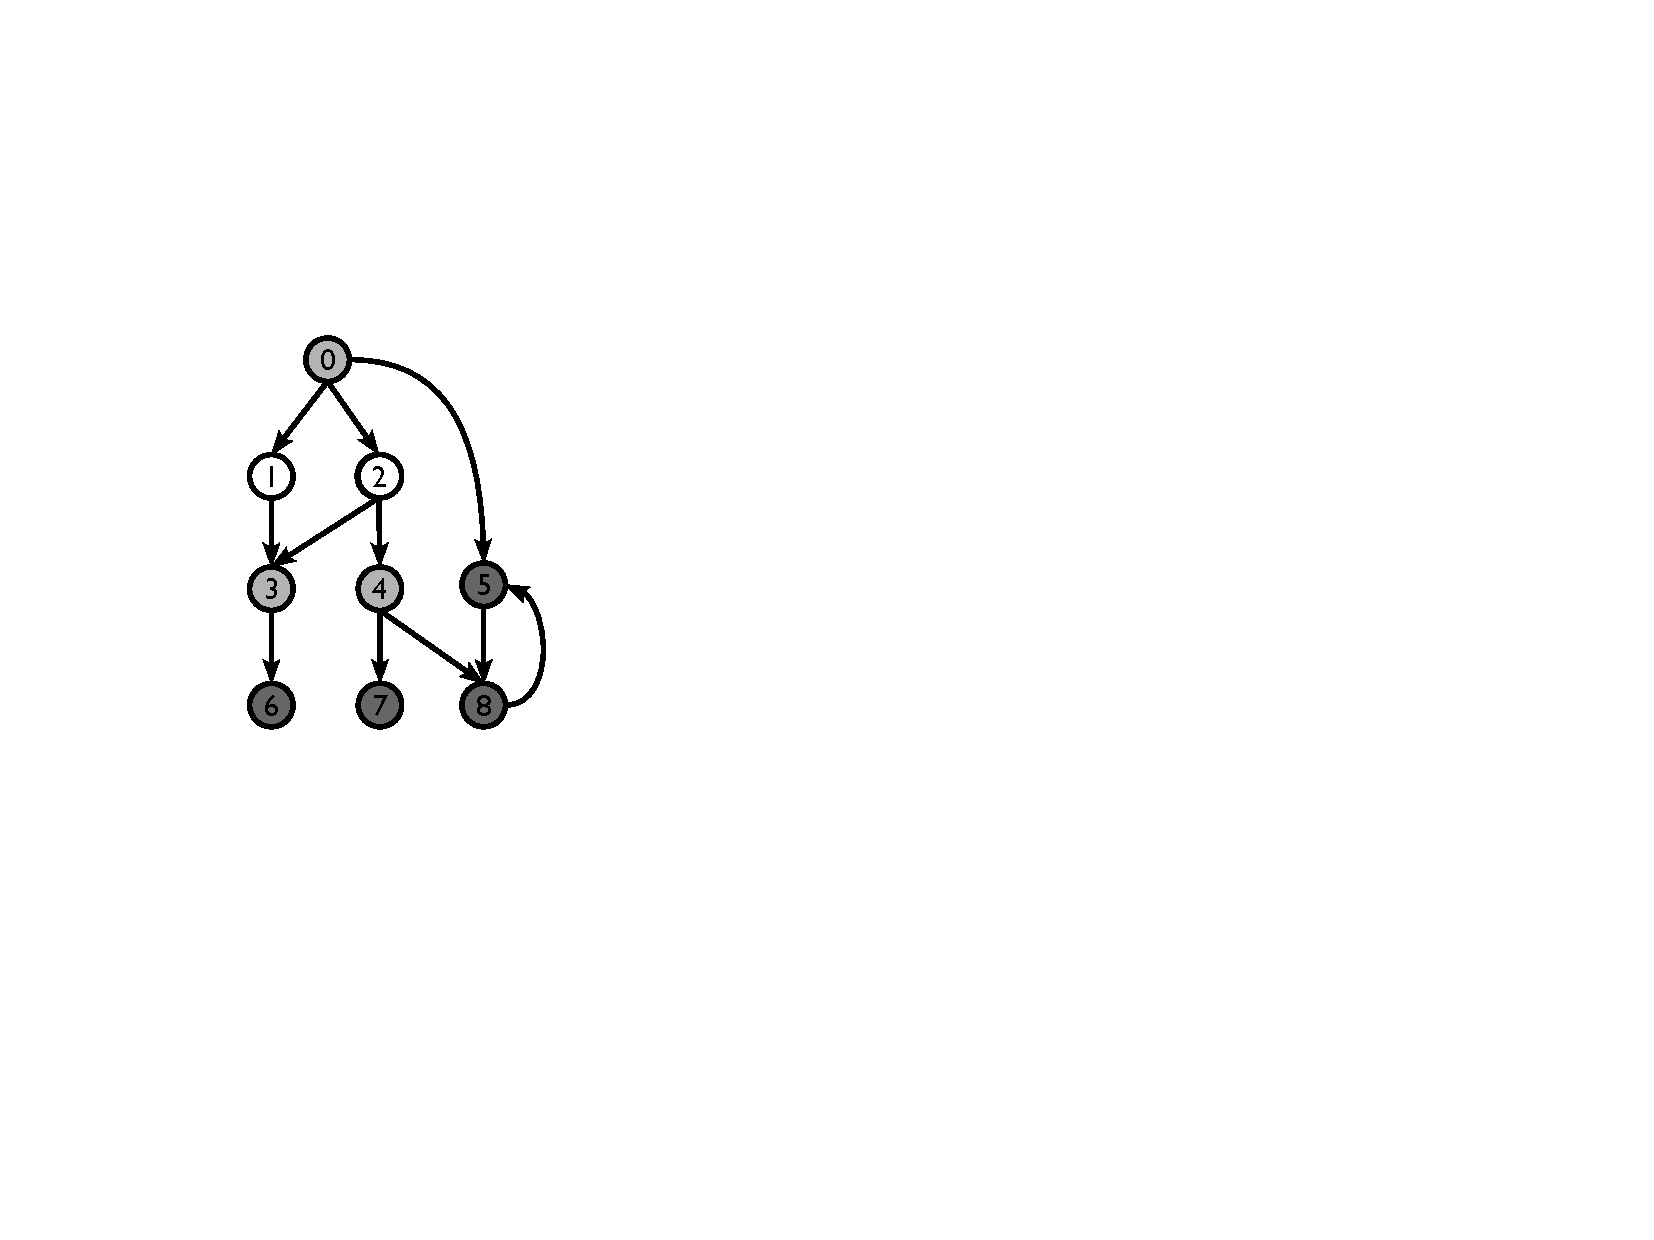
\includegraphics[width=0.3\textwidth]{part4/Figures/exampleGraph-withNodeNumbers}
}
\quad
\subfigure[The node attribute.]{
\shortstack{
\begin{tabular}{ll}
\multicolumn{1}{r}{\light{index}} & \multicolumn{1}{l}{\textbf{Color}}
\\ \toprule
\light{0} & LightGray \\ \midrule
\light{1} & White \\ \midrule
\light{2} & White \\ \midrule
\light{3} & LightGray \\ \midrule
\light{4} & LightGray \\ \midrule
\light{5} & DarkGray \\ \midrule
\light{6} & DarkGray \\ \midrule
\light{7} & DarkGray \\ \midrule
\light{8} & DarkGray \\
\bottomrule
\end{tabular}
\\ \vspace{0mm}
}
}
\quad
\subfigure[Edges.]{
\shortstack{
\begin{tabular}{r@{~~$\rightarrow$~~}l}
\textbf{from} & \textbf{to}
\\ \toprule
0 & 1 \\
0 & 2 \\
0 & 5 \\ \midrule
1 & 3 \\ \midrule
2 & 3 \\
2 & 4 \\ \midrule
3 & 6 \\ \midrule
4 & 7 \\
4 & 8 \\ \midrule
5 & 8 \\ \midrule
8 & 5 \\
\bottomrule
\end{tabular}
\\ \vspace{0mm}
}
}
\caption{A graph of nodes and edges can be represented
as a set of parallel arrays --- a column-oriented approach to storage, in the
style of Fortran. Edge attributes, along with additional node attributes, would
be stored in additional columns. The \light{index} column is not a stored
attribute, it is only shown in the table, for clarity.}
\label{fig:fortran-style}
\end{figure}

If you need the convenience of an actual \class{Node} object, you can have a
bit of both worlds. As long as you use the node objects
only for temporary purposes, then you have a good chance of avoiding a memory
footprint problem. These transient node objects act as facades to the
\class{NodeModel}, but require a reference to the \class{NodeModel} and the
node's index. 
\begin{shortlisting}
class TransientNode {
   NodeModel nodeModel;
   int nodeIndex;
   public Color getColor() {
      return nodeModel.getColor(nodeIndex);
   }
}
\end{shortlisting}
Though it has one extra field, on top of the earlier node implementations, for
the \class{NodeModel} reference, as long as it is transient, it could be fine.
This is something that requires experimentation in your setup. With transient
node facades, you are trading off more time spent in garbage collection for
convenience and the greater assurances you get from strong typing, compared to
passing around integers throughout your code, to represent node indices.
If these result in big drags in performance for your use cases, remember
that there is no absolute need for these transient node facades. You must also
be careful to either disallow, by convention, reference equality checks against
transient nodes, or cache any created objects.

The edges of a graph can be represented as two parallel arrays, storing the
source and target node indices of each edge, as shown in
\autoref{fig:fortran-style}c, and prototyped here:
\begin{shortlisting}
class EdgeModel {
   int[] from, to;
   public int getEdgeFrom(int i) {
      return from[i];
   }
   public int getEdgeTo(int i) {
      return to[i];
   }
}
\end{shortlisting}
However, this edge representation cannot efficiently support graph
traversals. There is no efficient way to retrieve the outgoing or
incoming edges from a given node. Even a \class{TransientEdge} class would not
help, because there is no connection between a node index and an index
into the edge model. Properly representing edges requires a bit more work. 

\paragraph{Representing Edges in a Column-oriented Storage Model}

To allow for efficient traversals of the edges, you must index them, as a
database would. First, consider the outgoing edges from a node. If the
\class{EdgeModel} parallel arrays are sorted by the \textbf{from} attribute, then
all of the children of a node will be stored contiguously. For example, the
edges in \autoref{fig:fortran-style}c have been sorted in this fashion.
At this point, it is
easy to establish an index, as an extra attribute of the \class{NodeModel}. This
attribute will store an index into this sorted edge model, which marks where the
children of each node begin. Once you have this index, then you no longer need to
store the \textbf{from} attribute in the edge model; it is implicit, in the
combination of the edge-start attribute of the node model. If you do so,
however, then you must also store the number of children of each node. 
\autoref{fig:fortran-style-edge-optimization} shows an update to
\autoref{fig:fortran-style}, where the node model now has, for the outgoing
edges, two new attributes: \textbf{EdgeStart} and \textbf{Num}. The same thing
can be done for the incoming edges, if we instead sort the edges of 
\autoref{fig:fortran-style}c by the \textbf{to} attribute.
\autoref{fig:fortran-style-edge-optimization}a also shows the two new attributes
for the incoming edges.  For example, node 2 has two children and
one parent. The children start at index 4 in
\autoref{fig:fortran-style-edge-optimization}b, which shows the two children to
be nodes 3 and 4.

\begin{figure}
\centering
\subfigure[Node attributes.]{
\shortstack{
\begin{tabular}{ll|ll|ll}
& & \multicolumn{2}{c|}{\textbf{Children}} &
\multicolumn{2}{c}{\textbf{Parents}} \\
\light{index} & \multicolumn{1}{l|}{\textbf{Color}} &
\multicolumn{1}{l}{\textbf{EdgeIndex}} & \multicolumn{1}{l|}{\textbf{Num}} & 
\multicolumn{1}{l}{\textbf{EdgeIndex}} &
\multicolumn{1}{l}{\textbf{Num}} \\ \toprule
\light{0} & LightGray & 0  & 3 & -- & 0 \\
\light{1} & White     & 3  & 1 & 0  & 1 \\
\light{2} & White     & 4  & 2 & 1  & 1 \\
\light{3} & LightGray & 6  & 1 & 2  & 2 \\
\light{4} & LightGray & 7  & 2 & 4  & 1 \\
\light{5} & DarkGray  & 9  & 1 & 5  & 2 \\
\light{6} & DarkGray  & -- & 0 & 7  & 1 \\
\light{7} & DarkGray  & -- & 0 & 8  & 1 \\
\light{8} & DarkGray  & 10 & 1 & 9  & 2 \\
\bottomrule
\end{tabular}
\\ \vspace{0mm}
}
}
\quad
\subfigure[Children edges.]{
\shortstack{
\begin{tabular}{ll}
\multicolumn{1}{r}{\light{index}} &
\multicolumn{1}{l}{\textbf{NodeIndex}} \\ \toprule
\light{0} & 1 \\
\light{1} & 2 \\
\light{2} & 5 \\ \midrule
\light{3} & 3 \\ \midrule
\light{4} & 3 \\
\light{5} & 4 \\ \midrule
\light{6} & 6 \\ \midrule
\light{7} & 7 \\
\light{8} & 8 \\ \midrule
\light{9} & 8 \\ \midrule
\light{10} & 5 \\
\bottomrule
\end{tabular}
\\ \vspace{0mm}
}
}
\quad
\subfigure[Parent edges.]{
\shortstack{
\begin{tabular}{ll}
\multicolumn{1}{r}{\light{index}} &
\multicolumn{1}{l}{\textbf{NodeIndex}}
\\ \toprule
\light{0} & 0 \\ \midrule  % 1 -> 0
\light{1} & 0 \\ \midrule  % 2 -> 0
\light{2} & 1 \\           % 3 -> 1
\light{3} & 2 \\ \midrule  % 3 -> 2
\light{4} & 2 \\ \midrule  % 4 -> 2
\light{5} & 0 \\ \midrule  % 5 -> 0
\light{6} & 8 \\           % 5 -> 8
\light{7} & 3 \\ \midrule  % 6 -> 3
\light{8} & 4 \\ \midrule  % 7 -> 4
\light{9} & 4 \\ \midrule  % 8 -> 4
\light{10} & 5 \\           % 8 -> 5
\bottomrule
\end{tabular}
\\ \vspace{0mm}
}
}
\caption{In order to support efficient traversal of the graph edges, you will
need to index them. These tables update the example of
\autoref{fig:fortran-style} to do so.  For example, node 2 has two children and
one parent. The children start at index 4 in
\autoref{fig:fortran-style-edge-optimization}b, which shows the two children to
be nodes 3 and 4.}
\label{fig:fortran-style-edge-optimization}
\end{figure}

\paragraph{Limitations of Column-oriented Storage}

There are two main problems you will run into, with a column-oriented approach.
The first has been touched on briefly: the lack of strong typing for nodes and
edges. If everything is just an integer, your code will be buggy and hard to
maintain. Java does not have a facility for naming types, such as \code{typedef}
in the C language. The Java \code{enum} construct seems like it could help, but
this use case would require a permanent object for every node, and, besides,
this construct is limited to around 65,000 entries per enumeration. You can use transient
nodes, with some cost to performance, but your code must still obey an implicit
contract, one not enforced by the \code{javac} compiler, that reference equality
is never used on these transient facades.

The second problem centers around modifications to the node or edge model. This
style of storage works fantasically well, much better than normal Java objects,
for certain kinds of modifications. Adding attributes to models is easy.
Adding nodes is straigtforward. However, deleting nodes, and adding or
removing edges from existing nodes can only be done with some extra work. For
deletions, you would have to implement a form of garbage collection yourself.
Nodes and edges can be marked as deleted; deleted elements would be ignored by
normal access mechanisms. Adding edges to existing nodes is even more difficult.
For these reasons, it is highly recommended that you only employ column-oriented
storage for data structures that do not change in these ways.

\section{Serialization}
\index{Serialization}

There are often situations where your data structures must be shuttled in and out
of the Java heap. Your application might be distributed across multiple boxes
that are connected by a network, rather than a distributed shared memory. It is
possible that your your data structures do not fit into available physical
memory, and so, rather than relying on the operating system's paging
functionality, you may find that you must implement a facility for doing so more
efficiently. Sometimes, you have enough physical memory, but are constrained by
available address space.\index{Address space exhasution} This is especially
likely to happen if you are running on a 32-bit \jre; e.g. if you run with a 1.5
gigabyte Java heap, and have one hundred thousand more more loaded classes, you
run the risk of exhausting the 2 gigabyte limit that most 32-bit operating
systems have, for each process. On many 32-bit versions of the Windows operating
system, and on 31-bit IBM mainframes, the address space limit is even lower than
2 gigabytes. It might also be that you have a need to perform relational queries
against your Java data structures, and are considering storing them in a
relational store to avoid having to implement the querying logic yourself. Your
reality might also be some combination of these.

It is important to remember that, in Java, the terms marshalling and
serialization are not synonymous. Serialization is the task of writing out the
bits, and the form of those bits. Marshalling, in the Java lexicon, is
serialization plus the assurance that all parties in the communication can agree
upon the version of the code that generated those bits. Without this agreement,
it can become difficult to manage evolving code bases, in the face of legacy
installations. This disparity of terminology is somewhat unique to Java, but the
distinction is nonetheless important. 

This book does not address the issues of compatibility of code bases, other than
to observe that, if your use case does not require handling code skew, then you
have options that will perform much better than using the built-in Java
marshalling mechanisms. In Java, there are several commonly available mechanisms
for marshalling your objects into and out of the Java heap. These include the
built-in Java object serialization, the Apache \class{XMLSerializer} and
\class{XMLDeserializer}. There is also a variety of libraries that provide a
mapping between Java objects and a relational backing store; an example is
RedHat's \class{Hibernate}. All of these come with a fair amount of expense,
because the \emph{operational} form of the data, that is the way the bits are
laid out as your Java code operates on them, is different from the serialized
form. Therefore, use of these serialization libraries usually entails an
expensive translation between two disparate storage formats.


\subsection{Memory Mapping}
\label{sec:memory-mapping}
\index{Memory Mapping}

One way to bring data in and out of Java without paying a marshalling expense
is via memory mapped I/O. When you \emph{memory map} a file into your address
space, you can treat the file as if it were an array. Reads and writes to the
array are reflected as disk reads or writes, and these operations are usually
done at a page granularity. Actual disk I/O may not occur with every array
access. This is the case if the operating system decides that it has enough
physical memory to keep the written pages in memory, and you haven't specified
that array writes should be written through to disk every time. Reads may be
serviced from this cache, as well. In this way, memory mapped I/O can have the
benefit of well-tested caching that balances that performance needs of all
processes running on your machine, without any work on your part.  Memory mapping
is a common trick used that is used by C programmers seeking the ultimate in
performance.

Since the cache is managed by the operating system, cached pages persist across
process boundaries. Therefore, if your application runs as multiple steps, each
in a separate process, then storing your data structures in memory mapped files
can result in a combination of caching and serialization-free persistence. The
unwritten buffers may eventually find their way to disk (if the underlying file
is not deleted first), but this needn't happen when one process terminates.

Used to its utmost, memory mapping can additionally offer one-copy bulk
transfers of memory to and from other processes, disk, or the network. For
example, say your application takes data from the network and writes it to
disk. If you memory map the network input buffers and the output file, and issue
bulk transfers from the input to the output, then it is possible that the
operating system will transfer the data directly from the network buffers to the
disk buffers, without first copying them out of the kernel, or into the
Java heap.

\paragraph{Memory Mapping in Java}
\index{\code{java.nio} library}
As of Java 1.4, a memory mapping facility is provided by the \code{java.nio}
library. This Java library manifests data as \class{ByteBuffer} objects. This
interface mimics an array, providing random access and bulk \code{get} and
\code{put} methods, but no insertion or deletion operations. Using this common
interface, you can access four repositories of data: network transmissions, files
on disk, memory allocations in the native heap, and allocations in the Java heap.
While the latter two can serve only as transient repositories for your data, they
avoid the expense of having to create a file on disk --- an expensive operation,
on most file systems, if done frequently.

You may find it useful to have the option to have some data stored in transient
storage, and others in persistent storage, backed by files on disk, and interact
with both using the same API. The \code{java.nio} library lets you do this. An
important advantage of using native \class{ByteBuffer} storage, over Java heap
storage, is that your application can run on arbitrarily large inputs without the
constraints of a fixed-maximum size Java heap.

No matter where the data is stored, you also have a choice of whether to use
standard Java byte ordering, or the byte ordering of the platform on which the
application is executing. Of course, this only matters if the data values you are
accessing are larger than a byte. On top of a \class{ByteBuffer}, you can layer
other primitive-type views. For example, the instance method
\code{ByteBuffer.asIntBuffer()} returns an \class{IntBuffer} that takes care of
any bit manipulations that are necessary to access the data as Java integers. If
you have chosen to use native byte ordering, then accessing the elements of an
\class{IntBuffer} on a 32-bit \jre requires no bit manipulation.

An example use of this library to create an integer array-like view over a file
is:

\begin{shortlisting}
IntBuffer mapAsIntegers(File file) {
   ByteBuffer buffer = new RandomAccessFile(file).getChannel().map(MapMode.READ_WRITE,0,file.length());
   // use platform, not Java, byte ordering
   buffer.order(ByteOrder.nativeOrder());
   return buffer.asIntBuffer();
}
\end{shortlisting}

\paragraph{Memory Mapping Your Column-oriented Storage}

There is a beneficial combination of memory mapping and a column-oriented
approach to storing your data. The interface to all memory mappings is an
array, and a column-oriented storage structure stores data as arrays. The
update, from the previous \class{EdgeModel} is easy, but requires a notion of a
namespace for each edge model. The namespace is necessary so that the model can
be mapped in from disk:

\begin{shortlisting}
class EdgeModel {
   IntBuffer from, to;
   public EdgeModel(File namespace) { // constructor
      from = mapAsIntegers(new File(namespace, "from"));
      to = mapAsIntegers(new File(namespace, "to"));
   }
   public int getEdgeFrom(int i) {
      return from.get(i);
   }
   public int getEdgeTo(int i) {
      return to.get(i);
   }
}
\end{shortlisting}

\paragraph{Difficulties with Memory Mapping in Java}

Each memory mapped file consumes only as much \emph{physical} memory as is
available and which the operating system decides, in its balancing act, is worthy
to allocate to the mapping. While all major operating system manage consumption
of physical memory, they do not similarly manage address space consumption. Thus,
each mapped \class{ByteBuffer} consumes a swath of address space equal to the
\emph{full} size of the map. For this reason, if you decide to use memory
mapping, you will run into several pernicious and interconnected problems. These
problems are orthogonal to any problems that stem from a choice to use
column-oriented storage.

The primary problem comes from the lack of an unmapping facility in the
\code{java.nio} library. You can not explicitly unmap a mapped area. Instead,
and, quite oddly, in direct contradiction of widely published best practices, the
library takes care of unmapping in the \code{finalize} method of the mapped
\class{ByteBuffer}. This leaves the timing of unmapping at the whim of garbage
collection and the subsequent scheduling of the finalizer thread. If you
application allocates very little in the way of temporary objects, but uses
memory mapping extensively, you will have failures due to address space
exhaustion. The garbage collector won't run, because plenty of Java heap is
available for allocation. However, memory mappings fail, because the process's
address space is fully consumed by older mappings, many of which would be
unmapped if the garbage collector were only to run.

This implementation decision has a strong negative interaction with the second
problem: the \jre does not, upon address space exhaustion, attempt to run a
garbage collection and finalization pass in order to clear out mapped byte
buffers. Therefore, you may suffer from \class{OutOfMemoryException} failures,
due to running out of address space, despite the fact that many of your mapped
regions are actually ready to be unmapped.

The third problem you may encounter is primarily to be found on Windows
platforms. The Windows operating system does not allow a file to be removed from
the file system if there are existing memory maps over any part of the file.
This, combined with the inability to explicitly unmap a mapping, can lead to a
situation where files remain on disk when you no longer need them. For example,
this can happen if there is a point in your code where you know the file is no
longer necessary, but there exist references from live objects or the stack to
the \class{ByteBuffer} object that represents the memory mapping. Since the
\class{ByteBuffer} facade is not garbage collectible, then its \code{finalize}
method will not be called, and hence the unmapping will not occur.

There is a set of policies you can follow to reduce the likelihood of such
problems. First, if possible, you should implement a correlated lifetime pattern
for the \class{ByteBuffer} objects. If these objects become garbage collectible
as soon as a phase or request completes, or correlated object is collected, then
the \code{ByteBuffer.finalize} method will be called as soon as possible after
that correlated event occurs. Next, you must trap all memory mapping failures,
force a garbage collection and finalization pass, and then retry the memory
mapping; doing this several times in a loop is recommended. Third, on some
versions of the \jre, you will find that a memory mapping failure results in the
\jre terminating the process. This was one, by the \jre developers, with the
thought that a memory mapping failure was a sign of catastrophic failure. You
know now that this is not the case, it is rather a symptom of the overall poor
design of the \code{java.nio} library. To work around this problem, you can set
up a security policy that disables calls to \code{System.exit}, though you must
be careful that your own code does not rely on this call.

The last good design principal, when using memory mapping in Java, is to rely on
file-based memory mappings as little as possible. If you need only temporary
mappings, then consider using the anonymous mappings described earlier:
\begin{shortlisting}
IntBuffer allocateAnonymousInts(int numBytes) {
   ByteBuffer buffer = ByteBuffer.allocateDirect(numBytes);
   buffer.order(ByteOrder.nativeOrder());
   return buffer.asIntBuffer();
}
\end{shortlisting}
When using anonymous maps, you must be aware of the default limits on these
native allocations. With Sun \jres, you can configure the maximum allowed number
of bytes allocated in this way via the command line argument
\code{-XX:MaxDirectMemorySize}; this option takes the same arguments as the
\code{-Xmx} setting. With IBM \jres, you do not need to specify a maximum value.


%\chapter{Lifetime Management in Other Languages}

\section{C++: Smart Pointers}

\code{auto\_ptr}, single-owner notion, auto-free

\section{C\#: Value Types}

\section{Ada95: Storage Pools}


%Bugs, performance problems, memory footprint.




%Story
%-------
%data has a natural lifetime
	%you can use the above mechanisms to manage
%sometimes we extend lifetime to optimize (for time)
%sometimes we shorten lifetime to optimize (for space)


%Problems:
	%Temps -- saving time
	%Making things fit
		%Things you need
		%Things you can recompute

		
		
		
%Chapter 1: Natural Lifetimes
	%- if scopes don't coincide with lifetime
	%- actual lifetime may be different from natural lifetime, for performance reasons
%Chapter 2: Getting Lifetime Correct
%Chapter 3: Getting It Small and Fast

